\documentclass[twoside]{book}

% Packages required by doxygen
\usepackage{calc}
\usepackage{doxygen}
\usepackage{graphicx}
\usepackage[utf8]{inputenc}
\usepackage{makeidx}
\usepackage{multicol}
\usepackage{multirow}
\usepackage{textcomp}
\usepackage[table]{xcolor}

% Font selection
\usepackage[T1]{fontenc}
\usepackage{mathptmx}
\usepackage[scaled=.90]{helvet}
\usepackage{courier}
\usepackage{amssymb}
\usepackage{sectsty}
\renewcommand{\familydefault}{\sfdefault}
\allsectionsfont{%
  \fontseries{bc}\selectfont%
  \color{darkgray}%
}
\renewcommand{\DoxyLabelFont}{%
  \fontseries{bc}\selectfont%
  \color{darkgray}%
}

% Page & text layout
\usepackage{geometry}
\geometry{%
  letterpaper,%
  top=2.5cm,%
  bottom=2.5cm,%
  left=2.5cm,%
  right=2.5cm%
}
\tolerance=750
\hfuzz=15pt
\hbadness=750
\setlength{\emergencystretch}{15pt}
\setlength{\parindent}{0cm}
\setlength{\parskip}{0.2cm}
\makeatletter
\renewcommand{\paragraph}{%
  \@startsection{paragraph}{4}{0ex}{-1.0ex}{1.0ex}{%
    \normalfont\normalsize\bfseries\SS@parafont%
  }%
}
\renewcommand{\subparagraph}{%
  \@startsection{subparagraph}{5}{0ex}{-1.0ex}{1.0ex}{%
    \normalfont\normalsize\bfseries\SS@subparafont%
  }%
}
\makeatother

% Headers & footers
\usepackage{fancyhdr}
\pagestyle{fancyplain}
\fancyhead[LE]{\fancyplain{}{\bfseries\thepage}}
\fancyhead[CE]{\fancyplain{}{}}
\fancyhead[RE]{\fancyplain{}{\bfseries\leftmark}}
\fancyhead[LO]{\fancyplain{}{\bfseries\rightmark}}
\fancyhead[CO]{\fancyplain{}{}}
\fancyhead[RO]{\fancyplain{}{\bfseries\thepage}}
\fancyfoot[LE]{\fancyplain{}{}}
\fancyfoot[CE]{\fancyplain{}{}}
\fancyfoot[RE]{\fancyplain{}{\bfseries\scriptsize Generated on Wed Apr 13 2016 22\-:43\-:55 for Lab 1 -\/ Motor Driver by Doxygen }}
\fancyfoot[LO]{\fancyplain{}{\bfseries\scriptsize Generated on Wed Apr 13 2016 22\-:43\-:55 for Lab 1 -\/ Motor Driver by Doxygen }}
\fancyfoot[CO]{\fancyplain{}{}}
\fancyfoot[RO]{\fancyplain{}{}}
\renewcommand{\footrulewidth}{0.4pt}
\renewcommand{\chaptermark}[1]{%
  \markboth{#1}{}%
}
\renewcommand{\sectionmark}[1]{%
  \markright{\thesection\ #1}%
}

% Indices & bibliography
\usepackage{natbib}
\usepackage[titles]{tocloft}
\setcounter{tocdepth}{3}
\setcounter{secnumdepth}{5}
\makeindex

% Hyperlinks (required, but should be loaded last)
\usepackage{ifpdf}
\ifpdf
  \usepackage[pdftex,pagebackref=true]{hyperref}
\else
  \usepackage[ps2pdf,pagebackref=true]{hyperref}
\fi
\hypersetup{%
  colorlinks=true,%
  linkcolor=blue,%
  citecolor=blue,%
  unicode%
}

% Custom commands
\newcommand{\clearemptydoublepage}{%
  \newpage{\pagestyle{empty}\cleardoublepage}%
}


%===== C O N T E N T S =====

\begin{document}

% Titlepage & ToC
\hypersetup{pageanchor=false}
\pagenumbering{roman}
\begin{titlepage}
\vspace*{7cm}
\begin{center}%
{\Large Lab 1 -\/ Motor Driver \\[1ex]\large 0.\-001 }\\
\vspace*{1cm}
{\large Generated by Doxygen 1.8.6}\\
\vspace*{0.5cm}
{\small Wed Apr 13 2016 22:43:55}\\
\end{center}
\end{titlepage}
\clearemptydoublepage
\tableofcontents
\clearemptydoublepage
\pagenumbering{arabic}
\hypersetup{pageanchor=true}

%--- Begin generated contents ---
\chapter{Hierarchical Index}
\section{Class Hierarchy}
This inheritance list is sorted roughly, but not completely, alphabetically\-:\begin{DoxyCompactList}
\item \contentsline{section}{adc}{\pageref{classadc}}{}
\item \contentsline{section}{pid\-:\-:config}{\pageref{structpid_1_1config}}{}
\item \contentsline{section}{encoder\-\_\-drv}{\pageref{classencoder__drv}}{}
\item \contentsline{section}{i2c\-\_\-master}{\pageref{classi2c__master}}{}
\item \contentsline{section}{imu\-\_\-drv}{\pageref{classimu__drv}}{}
\item \contentsline{section}{motor\-\_\-drv}{\pageref{classmotor__drv}}{}
\item \contentsline{section}{pid}{\pageref{classpid}}{}
\item Task\-Base\begin{DoxyCompactList}
\item \contentsline{section}{task\-\_\-encoder}{\pageref{classtask__encoder}}{}
\item \contentsline{section}{task\-\_\-imu}{\pageref{classtask__imu}}{}
\item \contentsline{section}{task\-\_\-motor}{\pageref{classtask__motor}}{}
\item \contentsline{section}{task\-\_\-pid}{\pageref{classtask__pid}}{}
\item \contentsline{section}{task\-\_\-user}{\pageref{classtask__user}}{}
\end{DoxyCompactList}
\end{DoxyCompactList}

\chapter{Class Index}
\section{Class List}
Here are the classes, structs, unions and interfaces with brief descriptions\-:\begin{DoxyCompactList}
\item\contentsline{section}{\hyperlink{classadc}{adc} \\*This define prevents this .H file from being included multiple times in a .C\-P\-P file }{\pageref{classadc}}{}
\item\contentsline{section}{\hyperlink{structpid_1_1config}{pid\-::config} \\*This struct defines a pid configuration }{\pageref{structpid_1_1config}}{}
\item\contentsline{section}{\hyperlink{classencoder__drv}{encoder\-\_\-drv} \\*This define prevents this .H file from being included multiple times in a .C\-P\-P file }{\pageref{classencoder__drv}}{}
\item\contentsline{section}{\hyperlink{classmotor__drv}{motor\-\_\-drv} \\*This define prevents this .H file from being included multiple times in a .C\-P\-P file }{\pageref{classmotor__drv}}{}
\item\contentsline{section}{\hyperlink{classpid}{pid} \\*This class runs a 16-\/bit fixed point P\-I\-D }{\pageref{classpid}}{}
\item\contentsline{section}{\hyperlink{classtask__encoder}{task\-\_\-encoder} \\*This define prevents this .H file from being included multiple times in a .C\-P\-P file }{\pageref{classtask__encoder}}{}
\item\contentsline{section}{\hyperlink{classtask__motor}{task\-\_\-motor} \\*This define prevents this .H file from being included multiple times in a .C\-P\-P file }{\pageref{classtask__motor}}{}
\item\contentsline{section}{\hyperlink{classtask__pid}{task\-\_\-pid} \\*This define prevents this .H file from being included multiple times in a .C\-P\-P file }{\pageref{classtask__pid}}{}
\item\contentsline{section}{\hyperlink{classtask__user}{task\-\_\-user} }{\pageref{classtask__user}}{}
\end{DoxyCompactList}

\chapter{File Index}
\section{File List}
Here is a list of all documented files with brief descriptions\-:\begin{DoxyCompactList}
\item\contentsline{section}{\hyperlink{adc_8cpp}{adc.\-cpp} }{\pageref{adc_8cpp}}{}
\item\contentsline{section}{\hyperlink{adc_8h}{adc.\-h} }{\pageref{adc_8h}}{}
\item\contentsline{section}{\hyperlink{encoder__drv_8cpp}{encoder\-\_\-drv.\-cpp} }{\pageref{encoder__drv_8cpp}}{}
\item\contentsline{section}{\hyperlink{encoder__drv_8h}{encoder\-\_\-drv.\-h} }{\pageref{encoder__drv_8h}}{}
\item\contentsline{section}{\hyperlink{main_8cpp}{main.\-cpp} }{\pageref{main_8cpp}}{}
\item\contentsline{section}{\hyperlink{motor__drv_8cpp}{motor\-\_\-drv.\-cpp} }{\pageref{motor__drv_8cpp}}{}
\item\contentsline{section}{\hyperlink{motor__drv_8h}{motor\-\_\-drv.\-h} }{\pageref{motor__drv_8h}}{}
\item\contentsline{section}{\hyperlink{pid_8cpp}{pid.\-cpp} }{\pageref{pid_8cpp}}{}
\item\contentsline{section}{\hyperlink{pid_8h}{pid.\-h} }{\pageref{pid_8h}}{}
\item\contentsline{section}{\hyperlink{satmath_8cpp}{satmath.\-cpp} }{\pageref{satmath_8cpp}}{}
\item\contentsline{section}{\hyperlink{satmath_8h}{satmath.\-h} }{\pageref{satmath_8h}}{}
\item\contentsline{section}{\hyperlink{shares_8h}{shares.\-h} }{\pageref{shares_8h}}{}
\item\contentsline{section}{\hyperlink{task__encoder_8cpp}{task\-\_\-encoder.\-cpp} }{\pageref{task__encoder_8cpp}}{}
\item\contentsline{section}{\hyperlink{task__encoder_8h}{task\-\_\-encoder.\-h} }{\pageref{task__encoder_8h}}{}
\item\contentsline{section}{\hyperlink{task__motor_8cpp}{task\-\_\-motor.\-cpp} }{\pageref{task__motor_8cpp}}{}
\item\contentsline{section}{\hyperlink{task__motor_8h}{task\-\_\-motor.\-h} }{\pageref{task__motor_8h}}{}
\item\contentsline{section}{\hyperlink{task__pid_8cpp}{task\-\_\-pid.\-cpp} }{\pageref{task__pid_8cpp}}{}
\item\contentsline{section}{\hyperlink{task__pid_8h}{task\-\_\-pid.\-h} }{\pageref{task__pid_8h}}{}
\item\contentsline{section}{\hyperlink{task__user_8cpp}{task\-\_\-user.\-cpp} }{\pageref{task__user_8cpp}}{}
\item\contentsline{section}{\hyperlink{task__user_8h}{task\-\_\-user.\-h} }{\pageref{task__user_8h}}{}
\end{DoxyCompactList}

\chapter{Class Documentation}
\hypertarget{classadc}{\section{adc Class Reference}
\label{classadc}\index{adc@{adc}}
}


This define prevents this .H file from being included multiple times in a .C\-P\-P file.  




{\ttfamily \#include $<$adc.\-h$>$}

\subsection*{Public Member Functions}
\begin{DoxyCompactItemize}
\item 
\hyperlink{classadc_af3b8262c08f5fc5ae325a20622883424}{adc} (emstream $\ast$=N\-U\-L\-L)
\begin{DoxyCompactList}\small\item\em This constructor sets up an A/\-D converter. \end{DoxyCompactList}\item 
uint16\-\_\-t \hyperlink{classadc_a2190a59696a7093e1ea605e998ccf97e}{read\-\_\-once} (uint8\-\_\-t)
\begin{DoxyCompactList}\small\item\em This method takes one A/\-D reading from the given channel and returns it. \end{DoxyCompactList}\item 
uint16\-\_\-t \hyperlink{classadc_a58f1030fe64d3dea4ccd8a2687dd6fce}{read\-\_\-oversampled} (uint8\-\_\-t, uint8\-\_\-t)
\begin{DoxyCompactList}\small\item\em This method takes a set number of A/\-D readings from a given channel and averages them. \end{DoxyCompactList}\end{DoxyCompactItemize}
\subsection*{Protected Attributes}
\begin{DoxyCompactItemize}
\item 
\hypertarget{classadc_a14680b48b723bf1adddd2741ebb18a3e}{emstream $\ast$ \hyperlink{classadc_a14680b48b723bf1adddd2741ebb18a3e}{ptr\-\_\-to\-\_\-serial}}\label{classadc_a14680b48b723bf1adddd2741ebb18a3e}

\begin{DoxyCompactList}\small\item\em The A\-D\-C class uses this pointer to the serial port to say hello. \end{DoxyCompactList}\end{DoxyCompactItemize}


\subsection{Detailed Description}
This define prevents this .H file from being included multiple times in a .C\-P\-P file. 

This class {\bfseries will} run the A/\-D converter on an A\-V\-R processor.

This class contains a pointer to the serial port, the constructor declaration for the A/\-D, a method that reads one sample of a A/\-D channel, and a method that reads a defined number of samples of a A/\-D channel. 

Definition at line 47 of file adc.\-h.



\subsection{Constructor \& Destructor Documentation}
\hypertarget{classadc_af3b8262c08f5fc5ae325a20622883424}{\index{adc@{adc}!adc@{adc}}
\index{adc@{adc}!adc@{adc}}
\subsubsection[{adc}]{\setlength{\rightskip}{0pt plus 5cm}adc\-::adc (
\begin{DoxyParamCaption}
\item[{emstream $\ast$}]{p\-\_\-serial\-\_\-port = {\ttfamily NULL}}
\end{DoxyParamCaption}
)}}\label{classadc_af3b8262c08f5fc5ae325a20622883424}


This constructor sets up an A/\-D converter. 

The constructor sets up the A/\-D converter for use. The \char`\"{}= N\-U\-L\-L\char`\"{} part is a default parameter, meaning that if that parameter isn't given on the line where this constructor is called, the compiler will just fill in \char`\"{}\-N\-U\-L\-L\char`\"{}. In this case that has the effect of turning off diagnostic printouts

The A/\-D is made ready so that when a method such as {\ttfamily \hyperlink{classadc_a2190a59696a7093e1ea605e998ccf97e}{read\-\_\-once()}} is called, correct A/\-D conversions can be performed. Enables the A/\-D converter, sets the clock prescaler to a divsion factor of 32, and selects reference voltage source as A\-V\-C\-C with external capactitor at A\-R\-E\-F pin. 
\begin{DoxyParams}{Parameters}
{\em p\-\_\-serial\-\_\-port} & A pointer to the serial port which writes debugging info. \\
\hline
\end{DoxyParams}


Definition at line 42 of file adc.\-cpp.



References ptr\-\_\-to\-\_\-serial.



\subsection{Member Function Documentation}
\hypertarget{classadc_a2190a59696a7093e1ea605e998ccf97e}{\index{adc@{adc}!read\-\_\-once@{read\-\_\-once}}
\index{read\-\_\-once@{read\-\_\-once}!adc@{adc}}
\subsubsection[{read\-\_\-once}]{\setlength{\rightskip}{0pt plus 5cm}uint16\-\_\-t adc\-::read\-\_\-once (
\begin{DoxyParamCaption}
\item[{uint8\-\_\-t}]{ch}
\end{DoxyParamCaption}
)}}\label{classadc_a2190a59696a7093e1ea605e998ccf97e}


This method takes one A/\-D reading from the given channel and returns it. 

This function reads one channel once, returning the result as an unsigned integer; it should be called from within a normal task, not an I\-S\-R

Forces the inputted channel to be a number from 0 to 7 then sets the A\-D\-M\-U\-X register to the correct channel. Next it starts the conversion and waits until it is finished. Finally it stores the result and returns it. 
\begin{DoxyParams}{Parameters}
{\em ch} & The A/\-D channel which is being read must be from 0 to 7 \\
\hline
\end{DoxyParams}
\begin{DoxyReturn}{Returns}
The result of the A/\-D conversion 
\end{DoxyReturn}


Definition at line 73 of file adc.\-cpp.



Referenced by operator$<$$<$(), and read\-\_\-oversampled().

\hypertarget{classadc_a58f1030fe64d3dea4ccd8a2687dd6fce}{\index{adc@{adc}!read\-\_\-oversampled@{read\-\_\-oversampled}}
\index{read\-\_\-oversampled@{read\-\_\-oversampled}!adc@{adc}}
\subsubsection[{read\-\_\-oversampled}]{\setlength{\rightskip}{0pt plus 5cm}uint16\-\_\-t adc\-::read\-\_\-oversampled (
\begin{DoxyParamCaption}
\item[{uint8\-\_\-t}]{channel, }
\item[{uint8\-\_\-t}]{samples}
\end{DoxyParamCaption}
)}}\label{classadc_a58f1030fe64d3dea4ccd8a2687dd6fce}


This method takes a set number of A/\-D readings from a given channel and averages them. 

This function reads the A/\-D lots of times and returns the average. Doing so implements a crude sort of low-\/pass filtering that can help reduce noise

Checks to see if number of samples inputted is above a threshold values then it takes samples and adds them up. Finally it returns the average of samples taken. 
\begin{DoxyParams}{Parameters}
{\em channel} & The A/\-D channel which is being read \\
\hline
{\em samples} & Number of samples to take for averaging reading \\
\hline
\end{DoxyParams}
\begin{DoxyReturn}{Returns}
Averaged result of A/\-D readings 
\end{DoxyReturn}


Definition at line 106 of file adc.\-cpp.



References read\-\_\-once().



The documentation for this class was generated from the following files\-:\begin{DoxyCompactItemize}
\item 
\hyperlink{adc_8h}{adc.\-h}\item 
\hyperlink{adc_8cpp}{adc.\-cpp}\end{DoxyCompactItemize}

\hypertarget{classmotor__drv}{\section{motor\-\_\-drv Class Reference}
\label{classmotor__drv}\index{motor\-\_\-drv@{motor\-\_\-drv}}
}


This class will enable the H-\/bridge motor driver chips on the M\-E 405 board.  




{\ttfamily \#include $<$motor\-\_\-drv.\-h$>$}

\subsection*{Public Member Functions}
\begin{DoxyCompactItemize}
\item 
\hyperlink{classmotor__drv_a13875fc8133ee2c8af383c4316278d84}{motor\-\_\-drv} (emstream $\ast$=N\-U\-L\-L, uint8\-\_\-t=0)
\begin{DoxyCompactList}\small\item\em This constructor sets up the motor object. \end{DoxyCompactList}\item 
void \hyperlink{classmotor__drv_a4b6d6fc9698bf76b9bf1bcbb660ad3b7}{set\-\_\-power} (int16\-\_\-t power)
\begin{DoxyCompactList}\small\item\em This method takes an integer and sets the motor torque and direction. \end{DoxyCompactList}\item 
void \hyperlink{classmotor__drv_ab9d99a1b71f8515240ff7748a16c937b}{brake\-\_\-full} ()
\begin{DoxyCompactList}\small\item\em This method causes the motor to brake fully. \end{DoxyCompactList}\item 
void \hyperlink{classmotor__drv_abf63b3c932b836bc3f97ebda5fd7e762}{brake} (uint8\-\_\-t strength)
\begin{DoxyCompactList}\small\item\em This method allows for the motor braking to be controlled. \end{DoxyCompactList}\end{DoxyCompactItemize}
\subsection*{Protected Attributes}
\begin{DoxyCompactItemize}
\item 
\hypertarget{classmotor__drv_a9cd3052255589d1849217279b4b6e337}{emstream $\ast$ {\bfseries ptr\-\_\-to\-\_\-serial}}\label{classmotor__drv_a9cd3052255589d1849217279b4b6e337}

\item 
\hypertarget{classmotor__drv_aca3c3dd889fd865607e312faf0e76c65}{uint8\-\_\-t {\bfseries select}}\label{classmotor__drv_aca3c3dd889fd865607e312faf0e76c65}

\end{DoxyCompactItemize}


\subsection{Detailed Description}
This class will enable the H-\/bridge motor driver chips on the M\-E 405 board. 

The class has two protected variables, one pointer that is used to print debug messages to the serial port and an select variable that is used to choose the appropriate registers for controlling the motor. The driver has three methods available to the user. The set\-\_\-power method allows the user to set the power supplied to the motor on a scale of -\/255 to 255 where the positive values turn the motor {\bfseries clockwise} and negative values turn the motor {\bfseries counterclockwise}. The brake\-\_\-full method effectively stops power being supplied to the motor. The brake method sets P\-W\-M controlled braking for motor. 

Definition at line 35 of file motor\-\_\-drv.\-h.



\subsection{Constructor \& Destructor Documentation}
\hypertarget{classmotor__drv_a13875fc8133ee2c8af383c4316278d84}{\index{motor\-\_\-drv@{motor\-\_\-drv}!motor\-\_\-drv@{motor\-\_\-drv}}
\index{motor\-\_\-drv@{motor\-\_\-drv}!motor_drv@{motor\-\_\-drv}}
\subsubsection[{motor\-\_\-drv}]{\setlength{\rightskip}{0pt plus 5cm}motor\-\_\-drv\-::motor\-\_\-drv (
\begin{DoxyParamCaption}
\item[{emstream $\ast$}]{p\-\_\-serial\-\_\-port = {\ttfamily NULL}, }
\item[{uint8\-\_\-t}]{motor\-\_\-select = {\ttfamily 0}}
\end{DoxyParamCaption}
)}}\label{classmotor__drv_a13875fc8133ee2c8af383c4316278d84}


This constructor sets up the motor object. 

The timer for the P\-W\-M signal is set up in fast P\-W\-M 8-\/bit mode with a clock prescaler of 8 which gives an operating frequency of approximately 8k\-Hz. The data direction registers and output enables are set for the appropriate motor based on the select variable. A debug message is printed stating if the motor constructor was sucessful or not. 
\begin{DoxyParams}{Parameters}
{\em p\-\_\-serial\-\_\-port} & A pointer to the serial port which writes debugging info. \\
\hline
{\em motor\-\_\-select} & Selects desired motor driver chip. \\
\hline
\end{DoxyParams}


Definition at line 28 of file motor\-\_\-drv.\-cpp.



\subsection{Member Function Documentation}
\hypertarget{classmotor__drv_abf63b3c932b836bc3f97ebda5fd7e762}{\index{motor\-\_\-drv@{motor\-\_\-drv}!brake@{brake}}
\index{brake@{brake}!motor_drv@{motor\-\_\-drv}}
\subsubsection[{brake}]{\setlength{\rightskip}{0pt plus 5cm}void motor\-\_\-drv\-::brake (
\begin{DoxyParamCaption}
\item[{uint8\-\_\-t}]{strength}
\end{DoxyParamCaption}
)}}\label{classmotor__drv_abf63b3c932b836bc3f97ebda5fd7e762}


This method allows for the motor braking to be controlled. 

The H-\/bridge chip for the corresponding motor is set to operating mode brake to G\-N\-D which allows for the use of the P\-W\-M signal to vary the braking strength. 
\begin{DoxyParams}{Parameters}
{\em strength} & Variable that sets amount of motor braking (must be between -\/255 and 255). \\
\hline
\end{DoxyParams}
\begin{DoxyReturn}{Returns}
None 
\end{DoxyReturn}


Definition at line 176 of file motor\-\_\-drv.\-cpp.

\hypertarget{classmotor__drv_ab9d99a1b71f8515240ff7748a16c937b}{\index{motor\-\_\-drv@{motor\-\_\-drv}!brake\-\_\-full@{brake\-\_\-full}}
\index{brake\-\_\-full@{brake\-\_\-full}!motor_drv@{motor\-\_\-drv}}
\subsubsection[{brake\-\_\-full}]{\setlength{\rightskip}{0pt plus 5cm}void motor\-\_\-drv\-::brake\-\_\-full (
\begin{DoxyParamCaption}
{}
\end{DoxyParamCaption}
)}}\label{classmotor__drv_ab9d99a1b71f8515240ff7748a16c937b}


This method causes the motor to brake fully. 

The H-\/bridge chip for the corresponding motor is set to operating mode brake to Vcc which effectively removes power from the motor causing it to brake. \begin{DoxyReturn}{Returns}
None 
\end{DoxyReturn}


Definition at line 151 of file motor\-\_\-drv.\-cpp.

\hypertarget{classmotor__drv_a4b6d6fc9698bf76b9bf1bcbb660ad3b7}{\index{motor\-\_\-drv@{motor\-\_\-drv}!set\-\_\-power@{set\-\_\-power}}
\index{set\-\_\-power@{set\-\_\-power}!motor_drv@{motor\-\_\-drv}}
\subsubsection[{set\-\_\-power}]{\setlength{\rightskip}{0pt plus 5cm}void motor\-\_\-drv\-::set\-\_\-power (
\begin{DoxyParamCaption}
\item[{int16\-\_\-t}]{power}
\end{DoxyParamCaption}
)}}\label{classmotor__drv_a4b6d6fc9698bf76b9bf1bcbb660ad3b7}


This method takes an integer and sets the motor torque and direction. 

The value of the integer corresponds to the amount of torque applied by the motor. The sign of the integer corresponds to the direction the motor turns. Negative values turn the motor {\bfseries clockwise} and positive values turn the motor {\bfseries counterclockwise}. 
\begin{DoxyParams}{Parameters}
{\em power} & Variable that sets power output to motor (must be between -\/255 and 255). \\
\hline
\end{DoxyParams}
\begin{DoxyReturn}{Returns}
None 
\end{DoxyReturn}


Definition at line 91 of file motor\-\_\-drv.\-cpp.



The documentation for this class was generated from the following files\-:\begin{DoxyCompactItemize}
\item 
\hyperlink{motor__drv_8h}{motor\-\_\-drv.\-h}\item 
\hyperlink{motor__drv_8cpp}{motor\-\_\-drv.\-cpp}\end{DoxyCompactItemize}

\hypertarget{classtask__brightness}{\section{task\-\_\-brightness Class Reference}
\label{classtask__brightness}\index{task\-\_\-brightness@{task\-\_\-brightness}}
}


This task controls the brightness of an L\-E\-D using an analog input from the A/\-D converter.  




{\ttfamily \#include $<$task\-\_\-brightness.\-h$>$}

Inheritance diagram for task\-\_\-brightness\-:\begin{figure}[H]
\begin{center}
\leavevmode
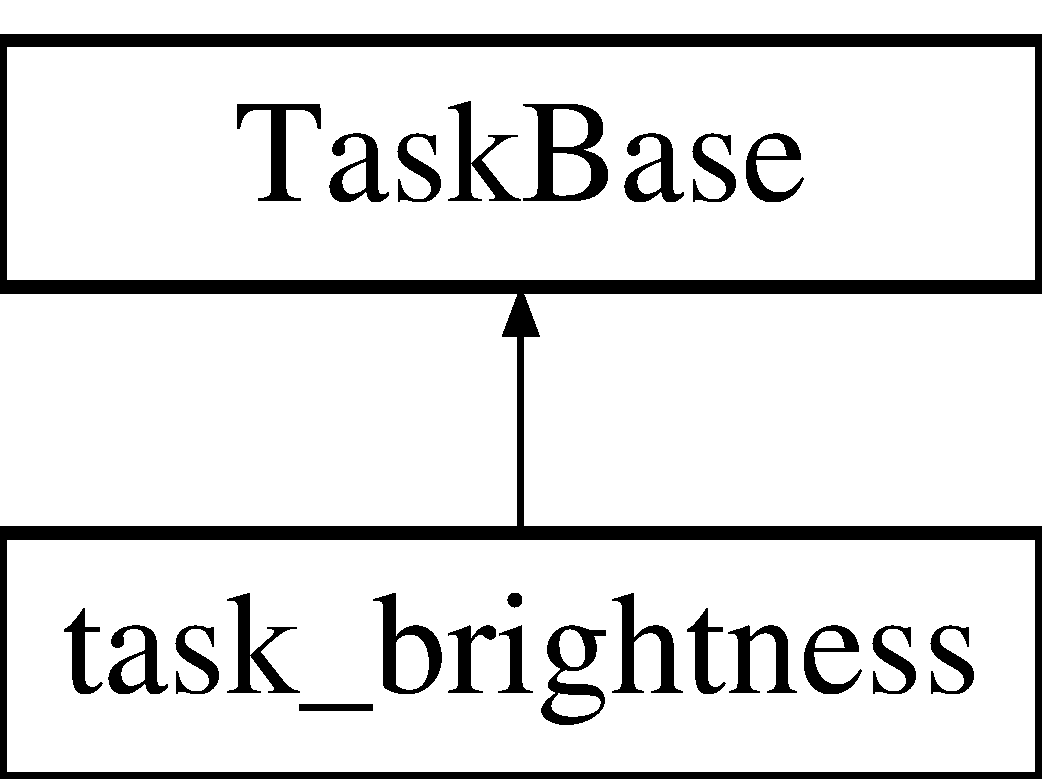
\includegraphics[height=2.000000cm]{classtask__brightness}
\end{center}
\end{figure}
\subsection*{Public Member Functions}
\begin{DoxyCompactItemize}
\item 
\hyperlink{classtask__brightness_a5802baf3a0c9fe53ccbce8966d1fad47}{task\-\_\-brightness} (const char $\ast$, unsigned port\-B\-A\-S\-E\-\_\-\-T\-Y\-P\-E, size\-\_\-t, emstream $\ast$)
\item 
void \hyperlink{classtask__brightness_a615beac07a99f0856f048a46fd9a3898}{run} (void)
\end{DoxyCompactItemize}


\subsection{Detailed Description}
This task controls the brightness of an L\-E\-D using an analog input from the A/\-D converter. 

The A/\-D converter is run using a driver in files {\ttfamily \hyperlink{adc_8h}{adc.\-h}} and {\ttfamily \hyperlink{adc_8cpp}{adc.\-cpp}}. Code in this task sets up a timer/counter in P\-W\-M mode and controls the L\-E\-D's average brightness. 

Definition at line 60 of file task\-\_\-brightness.\-h.



\subsection{Constructor \& Destructor Documentation}
\hypertarget{classtask__brightness_a5802baf3a0c9fe53ccbce8966d1fad47}{\index{task\-\_\-brightness@{task\-\_\-brightness}!task\-\_\-brightness@{task\-\_\-brightness}}
\index{task\-\_\-brightness@{task\-\_\-brightness}!task_brightness@{task\-\_\-brightness}}
\subsubsection[{task\-\_\-brightness}]{\setlength{\rightskip}{0pt plus 5cm}task\-\_\-brightness\-::task\-\_\-brightness (
\begin{DoxyParamCaption}
\item[{const char $\ast$}]{a\-\_\-name, }
\item[{unsigned port\-B\-A\-S\-E\-\_\-\-T\-Y\-P\-E}]{a\-\_\-priority, }
\item[{size\-\_\-t}]{a\-\_\-stack\-\_\-size, }
\item[{emstream $\ast$}]{p\-\_\-ser\-\_\-dev}
\end{DoxyParamCaption}
)}}\label{classtask__brightness_a5802baf3a0c9fe53ccbce8966d1fad47}
This constructor creates a task which controls the brightness of an L\-E\-D using input from an A/\-D converter. The main job of this constructor is to call the constructor of parent class ({\ttfamily frt\-\_\-task} ); the parent's constructor the work. 
\begin{DoxyParams}{Parameters}
{\em a\-\_\-name} & A character string which will be the name of this task \\
\hline
{\em a\-\_\-priority} & The priority at which this task will initially run (default\-: 0) \\
\hline
{\em a\-\_\-stack\-\_\-size} & The size of this task's stack in bytes (default\-: config\-M\-I\-N\-I\-M\-A\-L\-\_\-\-S\-T\-A\-C\-K\-\_\-\-S\-I\-Z\-E) \\
\hline
{\em p\-\_\-ser\-\_\-dev} & Pointer to a serial device (port, radio, S\-D card, etc.) which can be used by this task to communicate (default\-: N\-U\-L\-L) \\
\hline
\end{DoxyParams}


Definition at line 49 of file task\-\_\-brightness.\-cpp.



\subsection{Member Function Documentation}
\hypertarget{classtask__brightness_a615beac07a99f0856f048a46fd9a3898}{\index{task\-\_\-brightness@{task\-\_\-brightness}!run@{run}}
\index{run@{run}!task_brightness@{task\-\_\-brightness}}
\subsubsection[{run}]{\setlength{\rightskip}{0pt plus 5cm}void task\-\_\-brightness\-::run (
\begin{DoxyParamCaption}
\item[{void}]{}
\end{DoxyParamCaption}
)}}\label{classtask__brightness_a615beac07a99f0856f048a46fd9a3898}
This method is called once by the R\-T\-O\-S scheduler. Each time around the for (;;) loop, it reads the A/\-D converter and uses the result to control the brightness of an L\-E\-D. 

Definition at line 67 of file task\-\_\-brightness.\-cpp.



References adc\-::read\-\_\-once().



The documentation for this class was generated from the following files\-:\begin{DoxyCompactItemize}
\item 
\hyperlink{task__brightness_8h}{task\-\_\-brightness.\-h}\item 
\hyperlink{task__brightness_8cpp}{task\-\_\-brightness.\-cpp}\end{DoxyCompactItemize}

\hypertarget{classtask__motor}{\section{task\-\_\-motor Class Reference}
\label{classtask__motor}\index{task\-\_\-motor@{task\-\_\-motor}}
}


This define prevents this .H file from being included multiple times in a .C\-P\-P file.  




{\ttfamily \#include $<$task\-\_\-motor.\-h$>$}

Inheritance diagram for task\-\_\-motor\-:\begin{figure}[H]
\begin{center}
\leavevmode
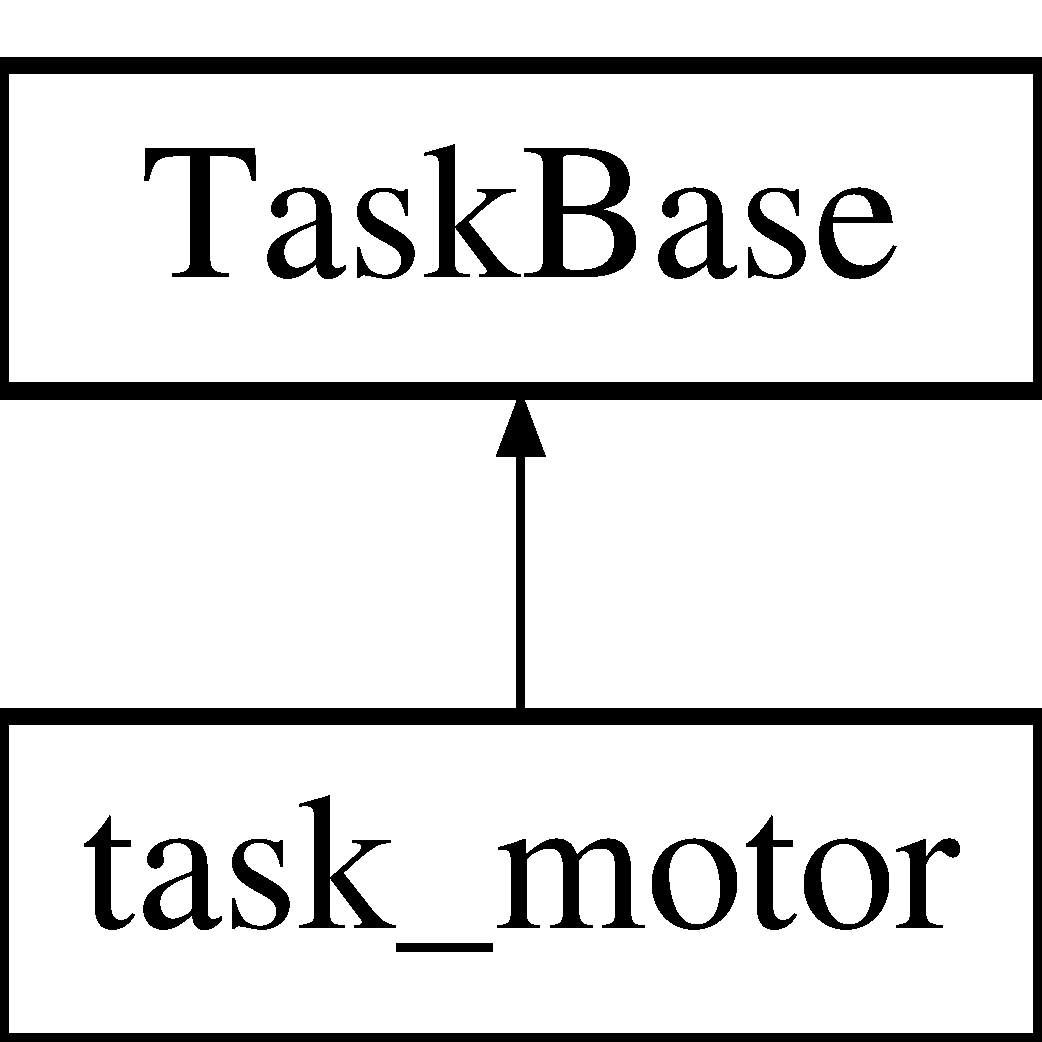
\includegraphics[height=2.000000cm]{classtask__motor}
\end{center}
\end{figure}
\subsection*{Public Member Functions}
\begin{DoxyCompactItemize}
\item 
\hyperlink{classtask__motor_a6ed0a0b463e698d636b28bcdd518a027}{task\-\_\-motor} (const char $\ast$, unsigned port\-B\-A\-S\-E\-\_\-\-T\-Y\-P\-E, size\-\_\-t, emstream $\ast$)
\begin{DoxyCompactList}\small\item\em No private variables or methods for this class. \end{DoxyCompactList}\item 
void \hyperlink{classtask__motor_a895a075ec470c9d5a07b8959de06aacd}{run} (void)
\begin{DoxyCompactList}\small\item\em This method is called by the R\-T\-O\-S once to run the task loop for ever and ever. \end{DoxyCompactList}\end{DoxyCompactItemize}


\subsection{Detailed Description}
This define prevents this .H file from being included multiple times in a .C\-P\-P file. 

Definition at line 33 of file task\-\_\-motor.\-h.



\subsection{Constructor \& Destructor Documentation}
\hypertarget{classtask__motor_a6ed0a0b463e698d636b28bcdd518a027}{\index{task\-\_\-motor@{task\-\_\-motor}!task\-\_\-motor@{task\-\_\-motor}}
\index{task\-\_\-motor@{task\-\_\-motor}!task_motor@{task\-\_\-motor}}
\subsubsection[{task\-\_\-motor}]{\setlength{\rightskip}{0pt plus 5cm}task\-\_\-motor\-::task\-\_\-motor (
\begin{DoxyParamCaption}
\item[{const char $\ast$}]{a\-\_\-name, }
\item[{unsigned port\-B\-A\-S\-E\-\_\-\-T\-Y\-P\-E}]{a\-\_\-priority, }
\item[{size\-\_\-t}]{a\-\_\-stack\-\_\-size, }
\item[{emstream $\ast$}]{p\-\_\-ser\-\_\-dev}
\end{DoxyParamCaption}
)}}\label{classtask__motor_a6ed0a0b463e698d636b28bcdd518a027}


No private variables or methods for this class. 

No protected variables or methods for this class This constructor creates a generic motor task of which many copies can be made.

This constructor creates a task which controls the ouput of two motors. The main job of this constructor is to call the constructor of parent class ({\ttfamily frt\-\_\-task} ); the parent's constructor the work. 
\begin{DoxyParams}{Parameters}
{\em a\-\_\-name} & A character string which will be the name of this task \\
\hline
{\em a\-\_\-priority} & The priority at which this task will initially run (default\-: 0) \\
\hline
{\em a\-\_\-stack\-\_\-size} & The size of this task's stack in bytes (default\-: config\-M\-I\-N\-I\-M\-A\-L\-\_\-\-S\-T\-A\-C\-K\-\_\-\-S\-I\-Z\-E) \\
\hline
{\em p\-\_\-ser\-\_\-dev} & Pointer to a serial device (port, radio, S\-D card, etc.) which can be used by this task to communicate (default\-: N\-U\-L\-L) \\
\hline
\end{DoxyParams}


Definition at line 29 of file task\-\_\-motor.\-cpp.



\subsection{Member Function Documentation}
\hypertarget{classtask__motor_a895a075ec470c9d5a07b8959de06aacd}{\index{task\-\_\-motor@{task\-\_\-motor}!run@{run}}
\index{run@{run}!task_motor@{task\-\_\-motor}}
\subsubsection[{run}]{\setlength{\rightskip}{0pt plus 5cm}void task\-\_\-motor\-::run (
\begin{DoxyParamCaption}
\item[{void}]{}
\end{DoxyParamCaption}
)}}\label{classtask__motor_a895a075ec470c9d5a07b8959de06aacd}


This method is called by the R\-T\-O\-S once to run the task loop for ever and ever. 

This method is called once by the R\-T\-O\-S scheduler. Each time around the for (;;) loop, it sets the power of the two motors and lets them run for two seconds then brakes them, waits for two seconds, and then runs them again in the opposite direction. 

Definition at line 42 of file task\-\_\-motor.\-cpp.



References sh\-\_\-braking\-\_\-entry, sh\-\_\-braking\-\_\-full\-\_\-flag, sh\-\_\-braking\-\_\-set\-\_\-flag, sh\-\_\-power\-\_\-entry, and sh\-\_\-power\-\_\-set\-\_\-flag.



The documentation for this class was generated from the following files\-:\begin{DoxyCompactItemize}
\item 
\hyperlink{task__motor_8h}{task\-\_\-motor.\-h}\item 
\hyperlink{task__motor_8cpp}{task\-\_\-motor.\-cpp}\end{DoxyCompactItemize}

\hypertarget{classtask__user}{\section{task\-\_\-user Class Reference}
\label{classtask__user}\index{task\-\_\-user@{task\-\_\-user}}
}


{\ttfamily \#include $<$task\-\_\-user.\-h$>$}

Inheritance diagram for task\-\_\-user\-:\begin{figure}[H]
\begin{center}
\leavevmode
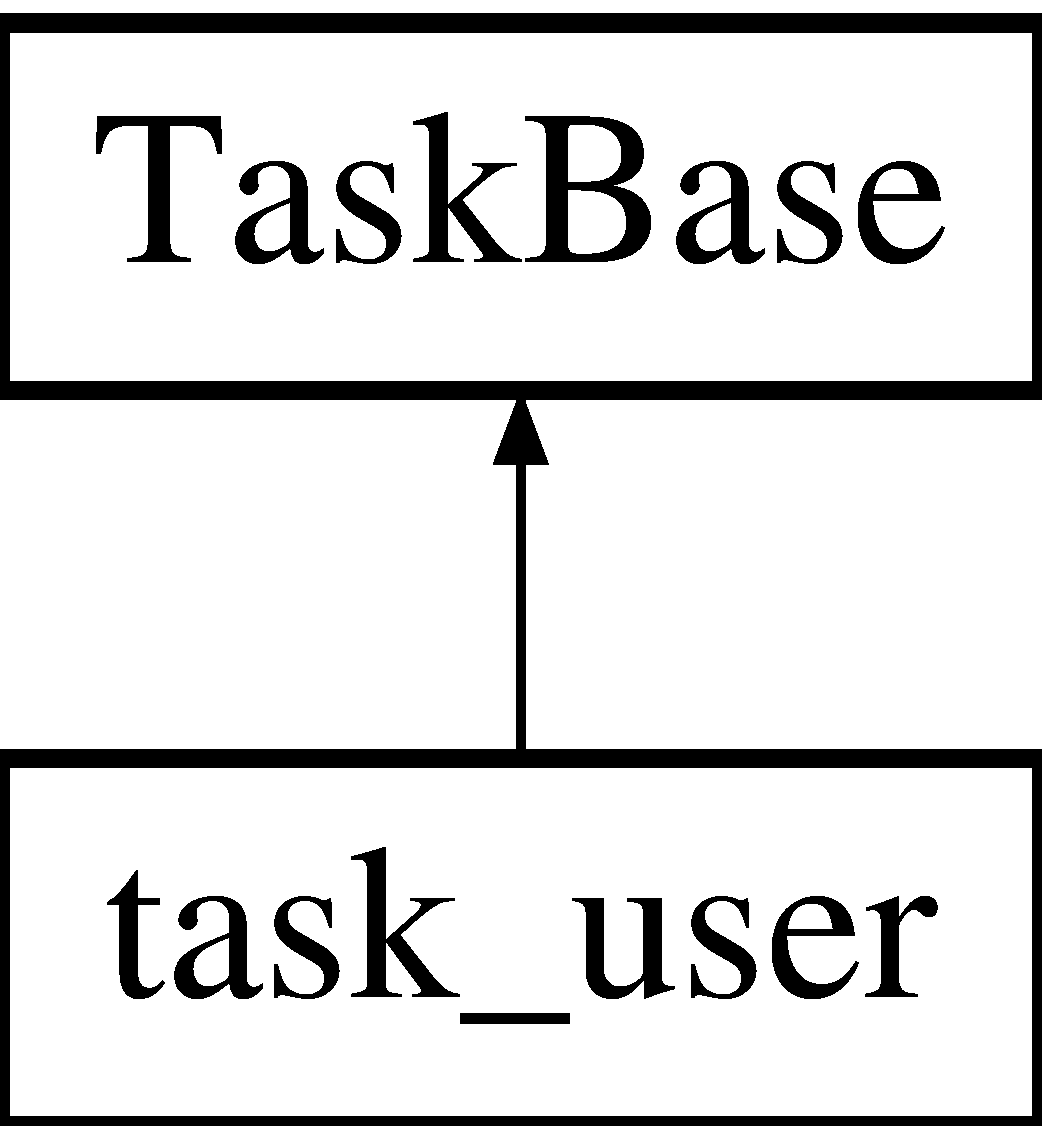
\includegraphics[height=2.000000cm]{classtask__user}
\end{center}
\end{figure}
\subsection*{Public Member Functions}
\begin{DoxyCompactItemize}
\item 
\hyperlink{classtask__user_a3aba77563b375bb14838800608da48bc}{task\-\_\-user} (const char $\ast$, unsigned port\-B\-A\-S\-E\-\_\-\-T\-Y\-P\-E, size\-\_\-t, emstream $\ast$)
\begin{DoxyCompactList}\small\item\em This constructor creates a user interface task object. \end{DoxyCompactList}\item 
void \hyperlink{classtask__user_adca6429d57be25e8d411414fc8ad75af}{run} (void)
\begin{DoxyCompactList}\small\item\em This method is called by the R\-T\-O\-S once to run the task loop for ever and ever. \end{DoxyCompactList}\end{DoxyCompactItemize}
\subsection*{Protected Member Functions}
\begin{DoxyCompactItemize}
\item 
\hypertarget{classtask__user_a36c99836d2ee036858d4a0ab61c2d5ec}{void \hyperlink{classtask__user_a36c99836d2ee036858d4a0ab61c2d5ec}{print\-\_\-main\-\_\-menu} (void)}\label{classtask__user_a36c99836d2ee036858d4a0ab61c2d5ec}

\begin{DoxyCompactList}\small\item\em This method displays the Main Menu message telling the user what to do. It's protected so that only methods of this class or possibly descendents can use it. \end{DoxyCompactList}\item 
\hypertarget{classtask__user_ae4c8890b06e117f57095951eee64c64f}{void \hyperlink{classtask__user_ae4c8890b06e117f57095951eee64c64f}{print\-\_\-motor\-\_\-menu} (void)}\label{classtask__user_ae4c8890b06e117f57095951eee64c64f}

\begin{DoxyCompactList}\small\item\em This method displays the Motor Menu message for motor control. It's protected so that only methods of this class or possibly descendents can use it. \end{DoxyCompactList}\item 
void \hyperlink{classtask__user_a105bebbd9cb1031154c3dfc3662db4a0}{show\-\_\-status} (void)
\begin{DoxyCompactList}\small\item\em This method displays information about the status of the system. \end{DoxyCompactList}\end{DoxyCompactItemize}


\subsection{Detailed Description}
This task interacts with the user for force him/her to do what he/she is told. What a rude task this is. Then again, computers tend to be that way; if they're polite with you, they're probably spying on you. 

Definition at line 57 of file task\-\_\-user.\-h.



\subsection{Constructor \& Destructor Documentation}
\hypertarget{classtask__user_a3aba77563b375bb14838800608da48bc}{\index{task\-\_\-user@{task\-\_\-user}!task\-\_\-user@{task\-\_\-user}}
\index{task\-\_\-user@{task\-\_\-user}!task_user@{task\-\_\-user}}
\subsubsection[{task\-\_\-user}]{\setlength{\rightskip}{0pt plus 5cm}task\-\_\-user\-::task\-\_\-user (
\begin{DoxyParamCaption}
\item[{const char $\ast$}]{a\-\_\-name, }
\item[{unsigned port\-B\-A\-S\-E\-\_\-\-T\-Y\-P\-E}]{a\-\_\-priority, }
\item[{size\-\_\-t}]{a\-\_\-stack\-\_\-size, }
\item[{emstream $\ast$}]{p\-\_\-ser\-\_\-dev}
\end{DoxyParamCaption}
)}}\label{classtask__user_a3aba77563b375bb14838800608da48bc}


This constructor creates a user interface task object. 

This constructor creates a new data acquisition task. It's main job is to call the parent class's constructor which does most of the work. 
\begin{DoxyParams}{Parameters}
{\em a\-\_\-name} & A character string which will be the name of this task \\
\hline
{\em a\-\_\-priority} & The priority at which this task will initially run (default\-: 0) \\
\hline
{\em a\-\_\-stack\-\_\-size} & The size of this task's stack in bytes (default\-: config\-M\-I\-N\-I\-M\-A\-L\-\_\-\-S\-T\-A\-C\-K\-\_\-\-S\-I\-Z\-E) \\
\hline
{\em p\-\_\-ser\-\_\-dev} & Pointer to a serial device (port, radio, S\-D card, etc.) which can be used by this task to communicate (default\-: N\-U\-L\-L) \\
\hline
\end{DoxyParams}


Definition at line 58 of file task\-\_\-user.\-cpp.



\subsection{Member Function Documentation}
\hypertarget{classtask__user_adca6429d57be25e8d411414fc8ad75af}{\index{task\-\_\-user@{task\-\_\-user}!run@{run}}
\index{run@{run}!task_user@{task\-\_\-user}}
\subsubsection[{run}]{\setlength{\rightskip}{0pt plus 5cm}void task\-\_\-user\-::run (
\begin{DoxyParamCaption}
\item[{void}]{}
\end{DoxyParamCaption}
)}}\label{classtask__user_adca6429d57be25e8d411414fc8ad75af}


This method is called by the R\-T\-O\-S once to run the task loop for ever and ever. 

This task interacts with the user so that a motor may be selected, the power for that motor may be set, the intensity of braking may also be set, along with a full braking option. It includes two help messages\-: Initial menu to choose global options, a motor menu to select power or braking intensity. T\-O\-D\-O\-: Add a increment and decrement for power increase Add a kill button to turn everything off if necessary 

Definition at line 74 of file task\-\_\-user.\-cpp.



References p\-\_\-print\-\_\-ser\-\_\-queue, print\-\_\-main\-\_\-menu(), print\-\_\-motor\-\_\-menu(), sh\-\_\-braking\-\_\-entry, sh\-\_\-braking\-\_\-full\-\_\-flag, sh\-\_\-braking\-\_\-set\-\_\-flag, sh\-\_\-motor\-\_\-select, sh\-\_\-power\-\_\-entry, sh\-\_\-power\-\_\-set\-\_\-flag, and show\-\_\-status().

\hypertarget{classtask__user_a105bebbd9cb1031154c3dfc3662db4a0}{\index{task\-\_\-user@{task\-\_\-user}!show\-\_\-status@{show\-\_\-status}}
\index{show\-\_\-status@{show\-\_\-status}!task_user@{task\-\_\-user}}
\subsubsection[{show\-\_\-status}]{\setlength{\rightskip}{0pt plus 5cm}void task\-\_\-user\-::show\-\_\-status (
\begin{DoxyParamCaption}
\item[{void}]{}
\end{DoxyParamCaption}
)\hspace{0.3cm}{\ttfamily [protected]}}}\label{classtask__user_a105bebbd9cb1031154c3dfc3662db4a0}


This method displays information about the status of the system. 

This method displays information about the status of the system, including the following\-: \begin{DoxyItemize}
\item The name and version of the program \item The name, status, priority, and free stack space of each task \item Processor cycles used by each task \item Amount of heap space free and setting of R\-T\-O\-S tick timer \end{DoxyItemize}


Definition at line 386 of file task\-\_\-user.\-cpp.



References P\-R\-O\-G\-R\-A\-M\-\_\-\-V\-E\-R\-S\-I\-O\-N.



Referenced by run().



The documentation for this class was generated from the following files\-:\begin{DoxyCompactItemize}
\item 
\hyperlink{task__user_8h}{task\-\_\-user.\-h}\item 
\hyperlink{task__user_8cpp}{task\-\_\-user.\-cpp}\end{DoxyCompactItemize}

\chapter{File Documentation}
\hypertarget{adc_8cpp}{\section{adc.\-cpp File Reference}
\label{adc_8cpp}\index{adc.\-cpp@{adc.\-cpp}}
}
{\ttfamily \#include $<$stdlib.\-h$>$}\\*
{\ttfamily \#include $<$avr/io.\-h$>$}\\*
{\ttfamily \#include \char`\"{}rs232int.\-h\char`\"{}}\\*
{\ttfamily \#include \char`\"{}adc.\-h\char`\"{}}\\*
\subsection*{Functions}
\begin{DoxyCompactItemize}
\item 
emstream \& \hyperlink{adc_8cpp_afb33ca9fe94765ee57079e7feb03f975}{operator$<$$<$} (emstream \&serpt, \hyperlink{classadc}{adc} \&a2d)
\begin{DoxyCompactList}\small\item\em This overloaded operator \char`\"{}prints the A/\-D converter.\char`\"{}. \end{DoxyCompactList}\end{DoxyCompactItemize}


\subsection{Detailed Description}
This file contains a very simple A/\-D converter driver.

Revisions\-: \begin{DoxyItemize}
\item 01-\/15-\/2008 J\-R\-R Original (somewhat useful) file \item 10-\/11-\/2012 J\-R\-R Less original, more useful file with Free\-R\-T\-O\-S mutex added \item 10-\/12-\/2012 J\-R\-R There was a bug in the mutex code, and it has been fixed\end{DoxyItemize}
License\-: This file is copyright 2015 by J\-R Ridgely and released under the Lesser G\-N\-U Public License, version 2. It intended for educational use only, but its use is not limited thereto. 

Definition in file \hyperlink{adc_8cpp_source}{adc.\-cpp}.



\subsection{Function Documentation}
\hypertarget{adc_8cpp_afb33ca9fe94765ee57079e7feb03f975}{\index{adc.\-cpp@{adc.\-cpp}!operator$<$$<$@{operator$<$$<$}}
\index{operator$<$$<$@{operator$<$$<$}!adc.cpp@{adc.\-cpp}}
\subsubsection[{operator$<$$<$}]{\setlength{\rightskip}{0pt plus 5cm}emstream\& operator$<$$<$ (
\begin{DoxyParamCaption}
\item[{emstream \&}]{serpt, }
\item[{{\bf adc} \&}]{a2d}
\end{DoxyParamCaption}
)}}\label{adc_8cpp_afb33ca9fe94765ee57079e7feb03f975}


This overloaded operator \char`\"{}prints the A/\-D converter.\char`\"{}. 

Prints out the value of the A\-D\-C\-S\-R\-A, A\-D\-M\-U\-X registers, and a single reading of channels 0 through 7 of the A/\-D. 
\begin{DoxyParams}{Parameters}
{\em serpt} & Reference to a serial port to which the printout will be printed \\
\hline
{\em a2d} & Reference to the A/\-D driver which is being printed \\
\hline
\end{DoxyParams}
\begin{DoxyReturn}{Returns}
A reference to the same serial device on which we write information. This is used to string together things to write with {\ttfamily $<$$<$} operators 
\end{DoxyReturn}


Definition at line 141 of file adc.\-cpp.



References adc\-::read\-\_\-once().


\hypertarget{adc_8h}{\section{adc.\-h File Reference}
\label{adc_8h}\index{adc.\-h@{adc.\-h}}
}
{\ttfamily \#include \char`\"{}emstream.\-h\char`\"{}}\\*
{\ttfamily \#include \char`\"{}Free\-R\-T\-O\-S.\-h\char`\"{}}\\*
{\ttfamily \#include \char`\"{}task.\-h\char`\"{}}\\*
{\ttfamily \#include \char`\"{}queue.\-h\char`\"{}}\\*
{\ttfamily \#include \char`\"{}semphr.\-h\char`\"{}}\\*
\subsection*{Classes}
\begin{DoxyCompactItemize}
\item 
class \hyperlink{classadc}{adc}
\begin{DoxyCompactList}\small\item\em This define prevents this .H file from being included multiple times in a .C\-P\-P file. \end{DoxyCompactList}\end{DoxyCompactItemize}
\subsection*{Functions}
\begin{DoxyCompactItemize}
\item 
emstream \& \hyperlink{adc_8h_a6e6d1e227b216fe2a1fee9b0ea52180d}{operator$<$$<$} (emstream \&, \hyperlink{classadc}{adc} \&)
\begin{DoxyCompactList}\small\item\em end of class adc \end{DoxyCompactList}\end{DoxyCompactItemize}


\subsection{Detailed Description}
This file contains a very simple A/\-D converter driver. The driver is hopefully thread safe in Free\-R\-T\-O\-S due to the use of a mutex to prevent its use by multiple tasks at the same time. There is no protection from priority inversion, however, except for the priority elevation in the mutex.

Revisions\-: \begin{DoxyItemize}
\item 01-\/15-\/2008 J\-R\-R Original (somewhat useful) file \item 10-\/11-\/2012 J\-R\-R Less original, more useful file with Free\-R\-T\-O\-S mutex added \item 10-\/12-\/2012 J\-R\-R There was a bug in the mutex code, and it has been fixed\end{DoxyItemize}
License\-: This file is copyright 2012 by J\-R Ridgely and released under the Lesser G\-N\-U Public License, version 2. It intended for educational use only, but its use is not limited thereto. 

Definition in file \hyperlink{adc_8h_source}{adc.\-h}.



\subsection{Function Documentation}
\hypertarget{adc_8h_a6e6d1e227b216fe2a1fee9b0ea52180d}{\index{adc.\-h@{adc.\-h}!operator$<$$<$@{operator$<$$<$}}
\index{operator$<$$<$@{operator$<$$<$}!adc.h@{adc.\-h}}
\subsubsection[{operator$<$$<$}]{\setlength{\rightskip}{0pt plus 5cm}emstream\& operator$<$$<$ (
\begin{DoxyParamCaption}
\item[{emstream \&}]{serpt, }
\item[{{\bf adc} \&}]{a2d}
\end{DoxyParamCaption}
)}}\label{adc_8h_a6e6d1e227b216fe2a1fee9b0ea52180d}


end of class adc 

This operator prints the A/\-D converter (see file \hyperlink{adc_8cpp}{adc.\-cpp} for details). It's not a part of class adc, but it operates on objects of class adc

end of class adc

Prints out the value of the A\-D\-C\-S\-R\-A, A\-D\-M\-U\-X registers, and a single reading of channels 0 through 7 of the A/\-D. 
\begin{DoxyParams}{Parameters}
{\em serpt} & Reference to a serial port to which the printout will be printed \\
\hline
{\em a2d} & Reference to the A/\-D driver which is being printed \\
\hline
\end{DoxyParams}
\begin{DoxyReturn}{Returns}
A reference to the same serial device on which we write information. This is used to string together things to write with {\ttfamily $<$$<$} operators 
\end{DoxyReturn}


Definition at line 141 of file adc.\-cpp.



References adc\-::read\-\_\-once().


\hypertarget{main_8cpp}{\section{main.\-cpp File Reference}
\label{main_8cpp}\index{main.\-cpp@{main.\-cpp}}
}
{\ttfamily \#include $<$stdlib.\-h$>$}\\*
{\ttfamily \#include $<$avr/io.\-h$>$}\\*
{\ttfamily \#include $<$avr/wdt.\-h$>$}\\*
{\ttfamily \#include $<$string.\-h$>$}\\*
{\ttfamily \#include \char`\"{}Free\-R\-T\-O\-S.\-h\char`\"{}}\\*
{\ttfamily \#include \char`\"{}task.\-h\char`\"{}}\\*
{\ttfamily \#include \char`\"{}queue.\-h\char`\"{}}\\*
{\ttfamily \#include \char`\"{}croutine.\-h\char`\"{}}\\*
{\ttfamily \#include \char`\"{}rs232int.\-h\char`\"{}}\\*
{\ttfamily \#include \char`\"{}time\-\_\-stamp.\-h\char`\"{}}\\*
{\ttfamily \#include \char`\"{}taskbase.\-h\char`\"{}}\\*
{\ttfamily \#include \char`\"{}textqueue.\-h\char`\"{}}\\*
{\ttfamily \#include \char`\"{}taskqueue.\-h\char`\"{}}\\*
{\ttfamily \#include \char`\"{}taskshare.\-h\char`\"{}}\\*
{\ttfamily \#include \char`\"{}shares.\-h\char`\"{}}\\*
{\ttfamily \#include \char`\"{}task\-\_\-user.\-h\char`\"{}}\\*
{\ttfamily \#include \char`\"{}motor\-\_\-drv.\-h\char`\"{}}\\*
{\ttfamily \#include \char`\"{}task\-\_\-motor.\-h\char`\"{}}\\*
{\ttfamily \#include \char`\"{}encoder\-\_\-drv.\-h\char`\"{}}\\*
{\ttfamily \#include \char`\"{}task\-\_\-encoder.\-h\char`\"{}}\\*
{\ttfamily \#include \char`\"{}task\-\_\-pid.\-h\char`\"{}}\\*
{\ttfamily \#include \char`\"{}pid.\-h\char`\"{}}\\*
\subsection*{Functions}
\begin{DoxyCompactItemize}
\item 
int \hyperlink{main_8cpp_a840291bc02cba5474a4cb46a9b9566fe}{main} (void)
\end{DoxyCompactItemize}
\subsection*{Variables}
\begin{DoxyCompactItemize}
\item 
Text\-Queue $\ast$ \hyperlink{main_8cpp_acd99bf5d187d4809af2f460a5415e904}{p\-\_\-print\-\_\-ser\-\_\-queue}
\begin{DoxyCompactList}\small\item\em This define prevents this .h file from being included multiple times in a .cpp file. \end{DoxyCompactList}\item 
\hypertarget{main_8cpp_a90445688792da1450704027ac2c4b6db}{Task\-Share$<$ int8\-\_\-t $>$ $\ast$ \hyperlink{main_8cpp_a90445688792da1450704027ac2c4b6db}{sh\-\_\-motor\-\_\-select}}\label{main_8cpp_a90445688792da1450704027ac2c4b6db}

\begin{DoxyCompactList}\small\item\em Motor selection share. \end{DoxyCompactList}\item 
\hypertarget{main_8cpp_a5cd0e4789d62c739a93ead239c5c42d8}{Task\-Share$<$ int16\-\_\-t $>$ $\ast$ \hyperlink{main_8cpp_a5cd0e4789d62c739a93ead239c5c42d8}{sh\-\_\-power\-\_\-entry}}\label{main_8cpp_a5cd0e4789d62c739a93ead239c5c42d8}

\begin{DoxyCompactList}\small\item\em Power value share. \end{DoxyCompactList}\item 
\hypertarget{main_8cpp_aacc570f48cbc8d62d6b506da980e5b36}{Task\-Share$<$ int8\-\_\-t $>$ $\ast$ \hyperlink{main_8cpp_aacc570f48cbc8d62d6b506da980e5b36}{sh\-\_\-power\-\_\-set\-\_\-flag}}\label{main_8cpp_aacc570f48cbc8d62d6b506da980e5b36}

\begin{DoxyCompactList}\small\item\em Flag share indicating power value has changed. \end{DoxyCompactList}\item 
\hypertarget{main_8cpp_a988f3cc5d8ffd96fed75760ef2b6cc12}{Task\-Share$<$ int16\-\_\-t $>$ $\ast$ \hyperlink{main_8cpp_a988f3cc5d8ffd96fed75760ef2b6cc12}{sh\-\_\-braking\-\_\-entry}}\label{main_8cpp_a988f3cc5d8ffd96fed75760ef2b6cc12}

\begin{DoxyCompactList}\small\item\em Braking value share. \end{DoxyCompactList}\item 
\hypertarget{main_8cpp_a23b68acc1e60935f6c5897a62b5b0221}{Task\-Share$<$ int8\-\_\-t $>$ $\ast$ \hyperlink{main_8cpp_a23b68acc1e60935f6c5897a62b5b0221}{sh\-\_\-braking\-\_\-set\-\_\-flag}}\label{main_8cpp_a23b68acc1e60935f6c5897a62b5b0221}

\begin{DoxyCompactList}\small\item\em Flag share indicating braking value has changed. \end{DoxyCompactList}\item 
\hypertarget{main_8cpp_a5aa2903e32574844afb823db851e91d8}{Task\-Share$<$ int8\-\_\-t $>$ $\ast$ \hyperlink{main_8cpp_a5aa2903e32574844afb823db851e91d8}{sh\-\_\-braking\-\_\-full\-\_\-flag}}\label{main_8cpp_a5aa2903e32574844afb823db851e91d8}

\begin{DoxyCompactList}\small\item\em Flag share indicating full braking requested. \end{DoxyCompactList}\item 
\hypertarget{main_8cpp_a997260f75507d382d25524c0b6716b9c}{Task\-Share$<$ volatile uint16\-\_\-t $>$ $\ast$ \hyperlink{main_8cpp_a997260f75507d382d25524c0b6716b9c}{sh\-\_\-encoder\-\_\-count\-\_\-1}}\label{main_8cpp_a997260f75507d382d25524c0b6716b9c}

\begin{DoxyCompactList}\small\item\em Encoder counts\-:Motor 1 encoder count. \end{DoxyCompactList}\item 
\hypertarget{main_8cpp_a88f2240863fddb31a613dded6ad871f8}{Task\-Share$<$ volatile uint16\-\_\-t $>$ $\ast$ \hyperlink{main_8cpp_a88f2240863fddb31a613dded6ad871f8}{sh\-\_\-encoder\-\_\-count\-\_\-2}}\label{main_8cpp_a88f2240863fddb31a613dded6ad871f8}

\begin{DoxyCompactList}\small\item\em Motor 1. \end{DoxyCompactList}\item 
Task\-Share$<$ volatile uint8\-\_\-t $>$ $\ast$ \hyperlink{main_8cpp_a1b679af79d73c380a7f0b4d49dcbc755}{sh\-\_\-encoder\-\_\-old\-\_\-state\-\_\-1}
\begin{DoxyCompactList}\small\item\em Motor 2. \end{DoxyCompactList}\item 
\hypertarget{main_8cpp_a777c7d499330fafba2cc196945515342}{Task\-Share$<$ volatile uint8\-\_\-t $>$ $\ast$ \hyperlink{main_8cpp_a777c7d499330fafba2cc196945515342}{sh\-\_\-encoder\-\_\-new\-\_\-state\-\_\-1}}\label{main_8cpp_a777c7d499330fafba2cc196945515342}

\begin{DoxyCompactList}\small\item\em Previous state. \end{DoxyCompactList}\item 
Task\-Share$<$ volatile uint8\-\_\-t $>$ $\ast$ \hyperlink{main_8cpp_af00b9d68b516e076df875afe7a1dfe96}{sh\-\_\-encoder\-\_\-old\-\_\-state\-\_\-2}
\begin{DoxyCompactList}\small\item\em Next state. \end{DoxyCompactList}\item 
\hypertarget{main_8cpp_a13e98b1ac77ef295fc268c40ce3cc94b}{Task\-Share$<$ volatile uint8\-\_\-t $>$ $\ast$ \hyperlink{main_8cpp_a13e98b1ac77ef295fc268c40ce3cc94b}{sh\-\_\-encoder\-\_\-new\-\_\-state\-\_\-2}}\label{main_8cpp_a13e98b1ac77ef295fc268c40ce3cc94b}

\begin{DoxyCompactList}\small\item\em Previous state. \end{DoxyCompactList}\item 
Task\-Share$<$ uint16\-\_\-t $>$ $\ast$ \hyperlink{main_8cpp_a1c714115d37fc602de04b1e93f2a63ae}{sh\-\_\-encoder\-\_\-error\-\_\-count\-\_\-1}
\begin{DoxyCompactList}\small\item\em Tick jump error count. \end{DoxyCompactList}\item 
\hypertarget{main_8cpp_a9ebd2476f8d88889d5a44476ca0db8fc}{Task\-Share$<$ uint16\-\_\-t $>$ $\ast$ {\bfseries sh\-\_\-encoder\-\_\-error\-\_\-count\-\_\-2}}\label{main_8cpp_a9ebd2476f8d88889d5a44476ca0db8fc}

\item 
\hypertarget{main_8cpp_a5e63825c91a8355dce1be62182669167}{Task\-Share$<$ volatile uint16\-\_\-t $>$ $\ast$ \hyperlink{main_8cpp_a5e63825c91a8355dce1be62182669167}{sh\-\_\-motor\-\_\-1\-\_\-speed}}\label{main_8cpp_a5e63825c91a8355dce1be62182669167}

\begin{DoxyCompactList}\small\item\em Next state. \end{DoxyCompactList}\item 
\hypertarget{main_8cpp_a6a429db733438657d6cda4d49a4d8eeb}{Task\-Share$<$ volatile uint16\-\_\-t $>$ $\ast$ \hyperlink{main_8cpp_a6a429db733438657d6cda4d49a4d8eeb}{sh\-\_\-motor\-\_\-2\-\_\-speed}}\label{main_8cpp_a6a429db733438657d6cda4d49a4d8eeb}

\begin{DoxyCompactList}\small\item\em Motor 1. \end{DoxyCompactList}\end{DoxyCompactItemize}


\subsection{Detailed Description}
This file contains the \hyperlink{main_8cpp_a840291bc02cba5474a4cb46a9b9566fe}{main()} code for a program which runs the M\-E405 board for M\-E405 lab 1. This program currently uses the H-\/bridge chips on the board to set the power of the two motors and let them run for two seconds then brakes them, waits for two seconds, and then runs them again in the opposite direction.

Revisions\-: \begin{DoxyItemize}
\item 09-\/30-\/2012 J\-R\-R Original file was a one-\/file demonstration with two tasks \item 10-\/05-\/2012 J\-R\-R Split into multiple files, one for each task plus a main one \item 10-\/30-\/2012 J\-R\-R A hopefully somewhat stable version with global queue pointers and the new operator used for most memory allocation \item 11-\/04-\/2012 J\-R\-R Free\-R\-T\-O\-S Swoop demo program changed to a sweet test suite \item 01-\/05-\/2012 J\-R\-R Program reconfigured as M\-E405 Lab 1 starting point \item 03-\/28-\/2014 J\-R\-R Pointers to shared variables and queues changed to references \item 01-\/04-\/2015 J\-R\-R Names of share \& queue classes changed; allocated with new now \item April 28, 2016 -- B\-K\-K Added shared variables (encoder\-: count, state, error count), commented out task\-\_\-brightness\-: was interfering with channel 4 interrupts.\end{DoxyItemize}
License\-: This file is copyright 2015 by J\-R Ridgely and released under the Lesser G\-N\-U Public License, version 2. It intended for educational use only, but its use is not limited thereto. T\-H\-I\-S S\-O\-F\-T\-W\-A\-R\-E I\-S P\-R\-O\-V\-I\-D\-E\-D B\-Y T\-H\-E C\-O\-P\-Y\-R\-I\-G\-H\-T H\-O\-L\-D\-E\-R\-S A\-N\-D C\-O\-N\-T\-R\-I\-B\-U\-T\-O\-R\-S \char`\"{}\-A\-S I\-S\char`\"{} A\-N\-D A\-N\-Y E\-X\-P\-R\-E\-S\-S O\-R I\-M\-P\-L\-I\-E\-D W\-A\-R\-R\-A\-N\-T\-I\-E\-S, I\-N\-C\-L\-U\-D\-I\-N\-G, B\-U\-T N\-O\-T L\-I\-M\-I\-T\-E\-D T\-O, T\-H\-E I\-M\-P\-L\-I\-E\-D W\-A\-R\-R\-A\-N\-T\-I\-E\-S O\-F M\-E\-R\-C\-H\-A\-N\-T\-A\-B\-I\-L\-I\-T\-Y A\-N\-D F\-I\-T\-N\-E\-S\-S F\-O\-R A P\-A\-R\-T\-I\-C\-U\-L\-A\-R P\-U\-R\-P\-O\-S\-E A\-R\-E D\-I\-S\-C\-L\-A\-I\-M\-E\-D. I\-N N\-O E\-V\-E\-N\-T S\-H\-A\-L\-L T\-H\-E C\-O\-P\-Y\-R\-I\-G\-H\-T O\-W\-N\-E\-R O\-R C\-O\-N\-T\-R\-I\-B\-U\-T\-O\-R\-S B\-E L\-I\-A\-B\-L\-E F\-O\-R A\-N\-Y D\-I\-R\-E\-C\-T, I\-N\-D\-I\-R\-E\-C\-T, I\-N\-C\-I\-D\-E\-N\-T\-A\-L, S\-P\-E\-C\-I\-A\-L, E\-X\-E\-M\-P\-L\-A\-R\-Y, O\-R C\-O\-N\-S\-E\-Q\-U\-E\-N\-T\-I\-A\-L D\-A\-M\-A\-G\-E\-S (I\-N\-C\-L\-U\-D\-I\-N\-G, B\-U\-T N\-O\-T L\-I\-M\-I\-T\-E\-D T\-O, P\-R\-O\-C\-U\-R\-E\-M\-E\-N\-T O\-F S\-U\-B\-S\-T\-I\-T\-U\-T\-E G\-O\-O\-D\-S O\-R S\-E\-R\-V\-I\-C\-E\-S; L\-O\-S\-S O\-F U\-S\-E, D\-A\-T\-A, O\-R P\-R\-O\-F\-I\-T\-S; O\-R B\-U\-S\-I\-N\-E\-S\-S I\-N\-T\-E\-R\-R\-U\-P\-T\-I\-O\-N) H\-O\-W\-E\-V\-E\-R C\-A\-U\-S\-E\-D A\-N\-D O\-N A\-N\-Y T\-H\-E\-O\-R\-Y O\-F L\-I\-A\-B\-I\-L\-I\-T\-Y, W\-H\-E\-T\-H\-E\-R I\-N C\-O\-N\-T\-R\-A\-C\-T, S\-T\-R\-I\-C\-T L\-I\-A\-B\-I\-L\-I\-T\-Y, O\-R T\-O\-R\-T (I\-N\-C\-L\-U\-D\-I\-N\-G N\-E\-G\-L\-I\-G\-E\-N\-C\-E O\-R O\-T\-H\-E\-R\-W\-I\-S\-E) A\-R\-I\-S\-I\-N\-G I\-N A\-N\-Y W\-A\-Y O\-U\-T O\-F T\-H\-E U\-S\-E O\-F T\-H\-I\-S S\-O\-F\-T\-W\-A\-R\-E, E\-V\-E\-N I\-F A\-D\-V\-I\-S\-E\-D O\-F T\-H\-E P\-O\-S\-S\-I\-B\-I\-L\-I\-T\-Y O\-F S\-U\-C\-H D\-A\-M\-A\-G\-E. 

Definition in file \hyperlink{main_8cpp_source}{main.\-cpp}.



\subsection{Function Documentation}
\hypertarget{main_8cpp_a840291bc02cba5474a4cb46a9b9566fe}{\index{main.\-cpp@{main.\-cpp}!main@{main}}
\index{main@{main}!main.cpp@{main.\-cpp}}
\subsubsection[{main}]{\setlength{\rightskip}{0pt plus 5cm}int main (
\begin{DoxyParamCaption}
\item[{void}]{}
\end{DoxyParamCaption}
)}}\label{main_8cpp_a840291bc02cba5474a4cb46a9b9566fe}
The main function sets up the R\-T\-O\-S. Some test tasks are created. Then the scheduler is started up; the scheduler runs until power is turned off or there's a reset. \begin{DoxyReturn}{Returns}
This is a real-\/time microcontroller program which doesn't return. 
\end{DoxyReturn}


Definition at line 104 of file main.\-cpp.



References p\-\_\-print\-\_\-ser\-\_\-queue, sh\-\_\-braking\-\_\-entry, sh\-\_\-braking\-\_\-full\-\_\-flag, sh\-\_\-braking\-\_\-set\-\_\-flag, sh\-\_\-encoder\-\_\-count\-\_\-1, sh\-\_\-encoder\-\_\-count\-\_\-2, sh\-\_\-encoder\-\_\-error\-\_\-count\-\_\-1, sh\-\_\-encoder\-\_\-new\-\_\-state\-\_\-1, sh\-\_\-encoder\-\_\-new\-\_\-state\-\_\-2, sh\-\_\-encoder\-\_\-old\-\_\-state\-\_\-1, sh\-\_\-encoder\-\_\-old\-\_\-state\-\_\-2, sh\-\_\-motor\-\_\-1\-\_\-speed, sh\-\_\-motor\-\_\-2\-\_\-speed, sh\-\_\-motor\-\_\-select, sh\-\_\-power\-\_\-entry, and sh\-\_\-power\-\_\-set\-\_\-flag.



\subsection{Variable Documentation}
\hypertarget{main_8cpp_acd99bf5d187d4809af2f460a5415e904}{\index{main.\-cpp@{main.\-cpp}!p\-\_\-print\-\_\-ser\-\_\-queue@{p\-\_\-print\-\_\-ser\-\_\-queue}}
\index{p\-\_\-print\-\_\-ser\-\_\-queue@{p\-\_\-print\-\_\-ser\-\_\-queue}!main.cpp@{main.\-cpp}}
\subsubsection[{p\-\_\-print\-\_\-ser\-\_\-queue}]{\setlength{\rightskip}{0pt plus 5cm}Text\-Queue$\ast$ p\-\_\-print\-\_\-ser\-\_\-queue}}\label{main_8cpp_acd99bf5d187d4809af2f460a5415e904}


This define prevents this .h file from being included multiple times in a .cpp file. 

This is a print queue, descended from {\ttfamily emstream} so that things can be printed into the queue using the \char`\"{}$<$$<$\char`\"{} operator and they'll come out the other end as a stream of characters. It's used by tasks that send things to the user interface task to be printed. 

Definition at line 70 of file main.\-cpp.



Referenced by main(), and task\-\_\-user\-::run().

\hypertarget{main_8cpp_a1c714115d37fc602de04b1e93f2a63ae}{\index{main.\-cpp@{main.\-cpp}!sh\-\_\-encoder\-\_\-error\-\_\-count\-\_\-1@{sh\-\_\-encoder\-\_\-error\-\_\-count\-\_\-1}}
\index{sh\-\_\-encoder\-\_\-error\-\_\-count\-\_\-1@{sh\-\_\-encoder\-\_\-error\-\_\-count\-\_\-1}!main.cpp@{main.\-cpp}}
\subsubsection[{sh\-\_\-encoder\-\_\-error\-\_\-count\-\_\-1}]{\setlength{\rightskip}{0pt plus 5cm}Task\-Share$<$uint16\-\_\-t$>$$\ast$ sh\-\_\-encoder\-\_\-error\-\_\-count\-\_\-1}}\label{main_8cpp_a1c714115d37fc602de04b1e93f2a63ae}


Tick jump error count. 

Motor 2 

Definition at line 92 of file main.\-cpp.



Referenced by I\-S\-R(), and main().

\hypertarget{main_8cpp_a1b679af79d73c380a7f0b4d49dcbc755}{\index{main.\-cpp@{main.\-cpp}!sh\-\_\-encoder\-\_\-old\-\_\-state\-\_\-1@{sh\-\_\-encoder\-\_\-old\-\_\-state\-\_\-1}}
\index{sh\-\_\-encoder\-\_\-old\-\_\-state\-\_\-1@{sh\-\_\-encoder\-\_\-old\-\_\-state\-\_\-1}!main.cpp@{main.\-cpp}}
\subsubsection[{sh\-\_\-encoder\-\_\-old\-\_\-state\-\_\-1}]{\setlength{\rightskip}{0pt plus 5cm}Task\-Share$<$volatile uint8\-\_\-t$>$$\ast$ sh\-\_\-encoder\-\_\-old\-\_\-state\-\_\-1}}\label{main_8cpp_a1b679af79d73c380a7f0b4d49dcbc755}


Motor 2. 

Motor 1 encoder states 

Definition at line 86 of file main.\-cpp.



Referenced by encoder\-\_\-drv\-::encoder\-\_\-drv(), I\-S\-R(), and main().

\hypertarget{main_8cpp_af00b9d68b516e076df875afe7a1dfe96}{\index{main.\-cpp@{main.\-cpp}!sh\-\_\-encoder\-\_\-old\-\_\-state\-\_\-2@{sh\-\_\-encoder\-\_\-old\-\_\-state\-\_\-2}}
\index{sh\-\_\-encoder\-\_\-old\-\_\-state\-\_\-2@{sh\-\_\-encoder\-\_\-old\-\_\-state\-\_\-2}!main.cpp@{main.\-cpp}}
\subsubsection[{sh\-\_\-encoder\-\_\-old\-\_\-state\-\_\-2}]{\setlength{\rightskip}{0pt plus 5cm}Task\-Share$<$volatile uint8\-\_\-t$>$$\ast$ sh\-\_\-encoder\-\_\-old\-\_\-state\-\_\-2}}\label{main_8cpp_af00b9d68b516e076df875afe7a1dfe96}


Next state. 

Motor 2 encoder states 

Definition at line 89 of file main.\-cpp.



Referenced by encoder\-\_\-drv\-::encoder\-\_\-drv(), I\-S\-R(), and main().


\hypertarget{motor__drv_8cpp}{\section{motor\-\_\-drv.\-cpp File Reference}
\label{motor__drv_8cpp}\index{motor\-\_\-drv.\-cpp@{motor\-\_\-drv.\-cpp}}
}
{\ttfamily \#include $<$stdlib.\-h$>$}\\*
{\ttfamily \#include $<$avr/io.\-h$>$}\\*
{\ttfamily \#include \char`\"{}rs232int.\-h\char`\"{}}\\*
{\ttfamily \#include \char`\"{}motor\-\_\-drv.\-h\char`\"{}}\\*


\subsection{Detailed Description}
This file contains the motor driver the two H-\/bridge chips on the M\-E 405 board.

Revisions\-: \begin{DoxyItemize}
\item 04-\/13-\/2016 M\-E405 Group 3 original file \end{DoxyItemize}


Definition in file \hyperlink{motor__drv_8cpp_source}{motor\-\_\-drv.\-cpp}.


\hypertarget{motor__drv_8h}{\section{motor\-\_\-drv.\-h File Reference}
\label{motor__drv_8h}\index{motor\-\_\-drv.\-h@{motor\-\_\-drv.\-h}}
}
{\ttfamily \#include \char`\"{}emstream.\-h\char`\"{}}\\*
{\ttfamily \#include \char`\"{}Free\-R\-T\-O\-S.\-h\char`\"{}}\\*
{\ttfamily \#include \char`\"{}task.\-h\char`\"{}}\\*
{\ttfamily \#include \char`\"{}queue.\-h\char`\"{}}\\*
{\ttfamily \#include \char`\"{}semphr.\-h\char`\"{}}\\*
\subsection*{Classes}
\begin{DoxyCompactItemize}
\item 
class \hyperlink{classmotor__drv}{motor\-\_\-drv}
\begin{DoxyCompactList}\small\item\em This define prevents this .H file from being included multiple times in a .C\-P\-P file. \end{DoxyCompactList}\end{DoxyCompactItemize}


\subsection{Detailed Description}
This file contains a simple motor driver that controls the two H-\/bridge chips on the M\-E 405 board.

Revisions\-: \begin{DoxyItemize}
\item 04-\/13-\/2016 M\-E405 Group 3 original file \end{DoxyItemize}


Definition in file \hyperlink{motor__drv_8h_source}{motor\-\_\-drv.\-h}.


\hypertarget{shares_8h}{\section{shares.\-h File Reference}
\label{shares_8h}\index{shares.\-h@{shares.\-h}}
}
\subsection*{Variables}
\begin{DoxyCompactItemize}
\item 
Text\-Queue $\ast$ \hyperlink{shares_8h_acd99bf5d187d4809af2f460a5415e904}{p\-\_\-print\-\_\-ser\-\_\-queue}
\begin{DoxyCompactList}\small\item\em This define prevents this .h file from being included multiple times in a .cpp file. \end{DoxyCompactList}\item 
\hypertarget{shares_8h_a90445688792da1450704027ac2c4b6db}{Task\-Share$<$ int8\-\_\-t $>$ $\ast$ \hyperlink{shares_8h_a90445688792da1450704027ac2c4b6db}{sh\-\_\-motor\-\_\-select}}\label{shares_8h_a90445688792da1450704027ac2c4b6db}

\begin{DoxyCompactList}\small\item\em Motor selection share. \end{DoxyCompactList}\item 
\hypertarget{shares_8h_a5cd0e4789d62c739a93ead239c5c42d8}{Task\-Share$<$ int16\-\_\-t $>$ $\ast$ \hyperlink{shares_8h_a5cd0e4789d62c739a93ead239c5c42d8}{sh\-\_\-power\-\_\-entry}}\label{shares_8h_a5cd0e4789d62c739a93ead239c5c42d8}

\begin{DoxyCompactList}\small\item\em Power value share. \end{DoxyCompactList}\item 
\hypertarget{shares_8h_aacc570f48cbc8d62d6b506da980e5b36}{Task\-Share$<$ int8\-\_\-t $>$ $\ast$ \hyperlink{shares_8h_aacc570f48cbc8d62d6b506da980e5b36}{sh\-\_\-power\-\_\-set\-\_\-flag}}\label{shares_8h_aacc570f48cbc8d62d6b506da980e5b36}

\begin{DoxyCompactList}\small\item\em Flag share indicating power value has changed. \end{DoxyCompactList}\item 
\hypertarget{shares_8h_a988f3cc5d8ffd96fed75760ef2b6cc12}{Task\-Share$<$ int16\-\_\-t $>$ $\ast$ \hyperlink{shares_8h_a988f3cc5d8ffd96fed75760ef2b6cc12}{sh\-\_\-braking\-\_\-entry}}\label{shares_8h_a988f3cc5d8ffd96fed75760ef2b6cc12}

\begin{DoxyCompactList}\small\item\em Braking value share. \end{DoxyCompactList}\item 
\hypertarget{shares_8h_a23b68acc1e60935f6c5897a62b5b0221}{Task\-Share$<$ int8\-\_\-t $>$ $\ast$ \hyperlink{shares_8h_a23b68acc1e60935f6c5897a62b5b0221}{sh\-\_\-braking\-\_\-set\-\_\-flag}}\label{shares_8h_a23b68acc1e60935f6c5897a62b5b0221}

\begin{DoxyCompactList}\small\item\em Flag share indicating braking value has changed. \end{DoxyCompactList}\item 
\hypertarget{shares_8h_a5aa2903e32574844afb823db851e91d8}{Task\-Share$<$ int8\-\_\-t $>$ $\ast$ \hyperlink{shares_8h_a5aa2903e32574844afb823db851e91d8}{sh\-\_\-braking\-\_\-full\-\_\-flag}}\label{shares_8h_a5aa2903e32574844afb823db851e91d8}

\begin{DoxyCompactList}\small\item\em Flag share indicating full braking requested. \end{DoxyCompactList}\item 
\hypertarget{shares_8h_a997260f75507d382d25524c0b6716b9c}{Task\-Share$<$ volatile uint16\-\_\-t $>$ $\ast$ \hyperlink{shares_8h_a997260f75507d382d25524c0b6716b9c}{sh\-\_\-encoder\-\_\-count\-\_\-1}}\label{shares_8h_a997260f75507d382d25524c0b6716b9c}

\begin{DoxyCompactList}\small\item\em Encoder counts\-:Motor 1 encoder count. \end{DoxyCompactList}\item 
\hypertarget{shares_8h_a88f2240863fddb31a613dded6ad871f8}{Task\-Share$<$ volatile uint16\-\_\-t $>$ $\ast$ \hyperlink{shares_8h_a88f2240863fddb31a613dded6ad871f8}{sh\-\_\-encoder\-\_\-count\-\_\-2}}\label{shares_8h_a88f2240863fddb31a613dded6ad871f8}

\begin{DoxyCompactList}\small\item\em Motor 1. \end{DoxyCompactList}\item 
Task\-Share$<$ volatile uint8\-\_\-t $>$ $\ast$ \hyperlink{shares_8h_a1b679af79d73c380a7f0b4d49dcbc755}{sh\-\_\-encoder\-\_\-old\-\_\-state\-\_\-1}
\begin{DoxyCompactList}\small\item\em Motor 2. \end{DoxyCompactList}\item 
\hypertarget{shares_8h_a777c7d499330fafba2cc196945515342}{Task\-Share$<$ volatile uint8\-\_\-t $>$ $\ast$ \hyperlink{shares_8h_a777c7d499330fafba2cc196945515342}{sh\-\_\-encoder\-\_\-new\-\_\-state\-\_\-1}}\label{shares_8h_a777c7d499330fafba2cc196945515342}

\begin{DoxyCompactList}\small\item\em Previous state. \end{DoxyCompactList}\item 
Task\-Share$<$ volatile uint8\-\_\-t $>$ $\ast$ \hyperlink{shares_8h_af00b9d68b516e076df875afe7a1dfe96}{sh\-\_\-encoder\-\_\-old\-\_\-state\-\_\-2}
\begin{DoxyCompactList}\small\item\em Next state. \end{DoxyCompactList}\item 
\hypertarget{shares_8h_a13e98b1ac77ef295fc268c40ce3cc94b}{Task\-Share$<$ volatile uint8\-\_\-t $>$ $\ast$ \hyperlink{shares_8h_a13e98b1ac77ef295fc268c40ce3cc94b}{sh\-\_\-encoder\-\_\-new\-\_\-state\-\_\-2}}\label{shares_8h_a13e98b1ac77ef295fc268c40ce3cc94b}

\begin{DoxyCompactList}\small\item\em Previous state. \end{DoxyCompactList}\item 
\hypertarget{shares_8h_a5e63825c91a8355dce1be62182669167}{Task\-Share$<$ volatile uint16\-\_\-t $>$ $\ast$ \hyperlink{shares_8h_a5e63825c91a8355dce1be62182669167}{sh\-\_\-motor\-\_\-1\-\_\-speed}}\label{shares_8h_a5e63825c91a8355dce1be62182669167}

\begin{DoxyCompactList}\small\item\em Next state. \end{DoxyCompactList}\item 
\hypertarget{shares_8h_a6a429db733438657d6cda4d49a4d8eeb}{Task\-Share$<$ volatile uint16\-\_\-t $>$ $\ast$ \hyperlink{shares_8h_a6a429db733438657d6cda4d49a4d8eeb}{sh\-\_\-motor\-\_\-2\-\_\-speed}}\label{shares_8h_a6a429db733438657d6cda4d49a4d8eeb}

\begin{DoxyCompactList}\small\item\em Motor 1. \end{DoxyCompactList}\item 
Task\-Share$<$ uint16\-\_\-t $>$ $\ast$ \hyperlink{shares_8h_a1c714115d37fc602de04b1e93f2a63ae}{sh\-\_\-encoder\-\_\-error\-\_\-count\-\_\-1}
\begin{DoxyCompactList}\small\item\em Tick jump error count. \end{DoxyCompactList}\item 
\hypertarget{shares_8h_a9ebd2476f8d88889d5a44476ca0db8fc}{Task\-Share$<$ uint16\-\_\-t $>$ $\ast$ {\bfseries sh\-\_\-encoder\-\_\-error\-\_\-count\-\_\-2}}\label{shares_8h_a9ebd2476f8d88889d5a44476ca0db8fc}

\end{DoxyCompactItemize}


\subsection{Detailed Description}
This file contains extern declarations for queues and other inter-\/task data communication objects used in a M\-E405/507/\-Free\-R\-T\-O\-S project.

Revisions\-: \begin{DoxyItemize}
\item 09-\/30-\/2012 J\-R\-R Original file was a one-\/file demonstration with two tasks \item 10-\/05-\/2012 J\-R\-R Split into multiple files, one for each task plus a main one \item 10-\/29-\/2012 J\-R\-R Reorganized with global queue and shared data references \item 01-\/04-\/2014 J\-R\-R Re-\/reorganized, allocating shares with new now \item April 28, 2016 -- B\-K\-K Added shared variables for encoder count, old and new state, error count\end{DoxyItemize}
License\-: This file is copyright 2015 by J\-R Ridgely and released under the Lesser G\-N\-U Public License, version 2. It intended for educational use only, but its use is not limited thereto. T\-H\-I\-S S\-O\-F\-T\-W\-A\-R\-E I\-S P\-R\-O\-V\-I\-D\-E\-D B\-Y T\-H\-E C\-O\-P\-Y\-R\-I\-G\-H\-T H\-O\-L\-D\-E\-R\-S A\-N\-D C\-O\-N\-T\-R\-I\-B\-U\-T\-O\-R\-S \char`\"{}\-A\-S I\-S\char`\"{} A\-N\-D A\-N\-Y E\-X\-P\-R\-E\-S\-S O\-R I\-M\-P\-L\-I\-E\-D W\-A\-R\-R\-A\-N\-T\-I\-E\-S, I\-N\-C\-L\-U\-D\-I\-N\-G, B\-U\-T N\-O\-T L\-I\-M\-I\-T\-E\-D T\-O, T\-H\-E I\-M\-P\-L\-I\-E\-D W\-A\-R\-R\-A\-N\-T\-I\-E\-S O\-F M\-E\-R\-C\-H\-A\-N\-T\-A\-B\-I\-L\-I\-T\-Y A\-N\-D F\-I\-T\-N\-E\-S\-S F\-O\-R A P\-A\-R\-T\-I\-C\-U\-L\-A\-R P\-U\-R\-P\-O\-S\-E A\-R\-E D\-I\-S\-C\-L\-A\-I\-M\-E\-D. I\-N N\-O E\-V\-E\-N\-T S\-H\-A\-L\-L T\-H\-E C\-O\-P\-Y\-R\-I\-G\-H\-T O\-W\-N\-E\-R O\-R C\-O\-N\-T\-R\-I\-B\-U\-T\-O\-R\-S B\-E L\-I\-A\-B\-L\-E F\-O\-R A\-N\-Y D\-I\-R\-E\-C\-T, I\-N\-D\-I\-R\-E\-C\-T, I\-N\-C\-I\-D\-E\-N\-T\-A\-L, S\-P\-E\-C\-I\-A\-L, E\-X\-E\-M\-P\-L\-A\-R\-Y, O\-R C\-O\-N\-S\-E\-Q\-U\-E\-N\-T\-I\-A\-L D\-A\-M\-A\-G\-E\-S (I\-N\-C\-L\-U\-D\-I\-N\-G, B\-U\-T N\-O\-T L\-I\-M\-I\-T\-E\-D T\-O, P\-R\-O\-C\-U\-R\-E\-M\-E\-N\-T O\-F S\-U\-B\-S\-T\-I\-T\-U\-T\-E G\-O\-O\-D\-S O\-R S\-E\-R\-V\-I\-C\-E\-S; L\-O\-S\-S O\-F U\-S\-E, D\-A\-T\-A, O\-R P\-R\-O\-F\-I\-T\-S; O\-R B\-U\-S\-I\-N\-E\-S\-S I\-N\-T\-E\-R\-R\-U\-P\-T\-I\-O\-N) H\-O\-W\-E\-V\-E\-R C\-A\-U\-S\-E\-D A\-N\-D O\-N A\-N\-Y T\-H\-E\-O\-R\-Y O\-F L\-I\-A\-B\-I\-L\-I\-T\-Y, W\-H\-E\-T\-H\-E\-R I\-N C\-O\-N\-T\-R\-A\-C\-T, S\-T\-R\-I\-C\-T L\-I\-A\-B\-I\-L\-I\-T\-Y, O\-R T\-O\-R\-T (I\-N\-C\-L\-U\-D\-I\-N\-G N\-E\-G\-L\-I\-G\-E\-N\-C\-E O\-R O\-T\-H\-E\-R\-W\-I\-S\-E) A\-R\-I\-S\-I\-N\-G I\-N A\-N\-Y W\-A\-Y O\-U\-T O\-F T\-H\-E U\-S\-E O\-F T\-H\-I\-S S\-O\-F\-T\-W\-A\-R\-E, E\-V\-E\-N I\-F A\-D\-V\-I\-S\-E\-D O\-F T\-H\-E P\-O\-S\-S\-I\-B\-I\-L\-I\-T\-Y O\-F S\-U\-C\-H D\-A\-M\-A\-G\-E. 

Definition in file \hyperlink{shares_8h_source}{shares.\-h}.



\subsection{Variable Documentation}
\hypertarget{shares_8h_acd99bf5d187d4809af2f460a5415e904}{\index{shares.\-h@{shares.\-h}!p\-\_\-print\-\_\-ser\-\_\-queue@{p\-\_\-print\-\_\-ser\-\_\-queue}}
\index{p\-\_\-print\-\_\-ser\-\_\-queue@{p\-\_\-print\-\_\-ser\-\_\-queue}!shares.h@{shares.\-h}}
\subsubsection[{p\-\_\-print\-\_\-ser\-\_\-queue}]{\setlength{\rightskip}{0pt plus 5cm}Text\-Queue$\ast$ p\-\_\-print\-\_\-ser\-\_\-queue}}\label{shares_8h_acd99bf5d187d4809af2f460a5415e904}


This define prevents this .h file from being included multiple times in a .cpp file. 

Externs\-: In this section, we declare variables and functions that are used in all (or at least two) of the files in the data acquisition project. Each of these items will also be declared exactly once, without the keyword 'extern', in one .cpp file as well as being declared extern here. This queue allows tasks to send characters to the user interface task for display.

This is a print queue, descended from {\ttfamily emstream} so that things can be printed into the queue using the \char`\"{}$<$$<$\char`\"{} operator and they'll come out the other end as a stream of characters. It's used by tasks that send things to the user interface task to be printed. 

Definition at line 66 of file main.\-cpp.



Referenced by main(), and task\-\_\-user\-::run().

\hypertarget{shares_8h_a1c714115d37fc602de04b1e93f2a63ae}{\index{shares.\-h@{shares.\-h}!sh\-\_\-encoder\-\_\-error\-\_\-count\-\_\-1@{sh\-\_\-encoder\-\_\-error\-\_\-count\-\_\-1}}
\index{sh\-\_\-encoder\-\_\-error\-\_\-count\-\_\-1@{sh\-\_\-encoder\-\_\-error\-\_\-count\-\_\-1}!shares.h@{shares.\-h}}
\subsubsection[{sh\-\_\-encoder\-\_\-error\-\_\-count\-\_\-1}]{\setlength{\rightskip}{0pt plus 5cm}Task\-Share$<$uint16\-\_\-t$>$$\ast$ sh\-\_\-encoder\-\_\-error\-\_\-count\-\_\-1}}\label{shares_8h_a1c714115d37fc602de04b1e93f2a63ae}


Tick jump error count. 

Motor 2 

Definition at line 88 of file main.\-cpp.



Referenced by I\-S\-R(), and main().

\hypertarget{shares_8h_a1b679af79d73c380a7f0b4d49dcbc755}{\index{shares.\-h@{shares.\-h}!sh\-\_\-encoder\-\_\-old\-\_\-state\-\_\-1@{sh\-\_\-encoder\-\_\-old\-\_\-state\-\_\-1}}
\index{sh\-\_\-encoder\-\_\-old\-\_\-state\-\_\-1@{sh\-\_\-encoder\-\_\-old\-\_\-state\-\_\-1}!shares.h@{shares.\-h}}
\subsubsection[{sh\-\_\-encoder\-\_\-old\-\_\-state\-\_\-1}]{\setlength{\rightskip}{0pt plus 5cm}Task\-Share$<$volatile uint8\-\_\-t$>$$\ast$ sh\-\_\-encoder\-\_\-old\-\_\-state\-\_\-1}}\label{shares_8h_a1b679af79d73c380a7f0b4d49dcbc755}


Motor 2. 

Motor 1 encoder states 

Definition at line 82 of file main.\-cpp.



Referenced by encoder\-\_\-drv\-::encoder\-\_\-drv(), I\-S\-R(), and main().

\hypertarget{shares_8h_af00b9d68b516e076df875afe7a1dfe96}{\index{shares.\-h@{shares.\-h}!sh\-\_\-encoder\-\_\-old\-\_\-state\-\_\-2@{sh\-\_\-encoder\-\_\-old\-\_\-state\-\_\-2}}
\index{sh\-\_\-encoder\-\_\-old\-\_\-state\-\_\-2@{sh\-\_\-encoder\-\_\-old\-\_\-state\-\_\-2}!shares.h@{shares.\-h}}
\subsubsection[{sh\-\_\-encoder\-\_\-old\-\_\-state\-\_\-2}]{\setlength{\rightskip}{0pt plus 5cm}Task\-Share$<$volatile uint8\-\_\-t$>$$\ast$ sh\-\_\-encoder\-\_\-old\-\_\-state\-\_\-2}}\label{shares_8h_af00b9d68b516e076df875afe7a1dfe96}


Next state. 

Motor 2 encoder states 

Definition at line 85 of file main.\-cpp.



Referenced by encoder\-\_\-drv\-::encoder\-\_\-drv(), I\-S\-R(), and main().


\hypertarget{task__brightness_8cpp}{\section{task\-\_\-brightness.\-cpp File Reference}
\label{task__brightness_8cpp}\index{task\-\_\-brightness.\-cpp@{task\-\_\-brightness.\-cpp}}
}
{\ttfamily \#include \char`\"{}textqueue.\-h\char`\"{}}\\*
{\ttfamily \#include \char`\"{}task\-\_\-brightness.\-h\char`\"{}}\\*
{\ttfamily \#include \char`\"{}shares.\-h\char`\"{}}\\*


\subsection{Detailed Description}
This file contains the code for a task class which controls the brightness of an L\-E\-D using a voltage measured from the A/\-D as input. The fun part\-: the brightness that is being controlled can be on another A\-V\-R computer, with signals being sent and received via wireless transceivers.

Revisions\-: \begin{DoxyItemize}
\item 09-\/30-\/2012 J\-R\-R Original file was a one-\/file demonstration with two tasks \item 10-\/05-\/2012 J\-R\-R Split into multiple files, one for each task \item 10-\/25-\/2012 J\-R\-R Changed to a more fully C++ version with class task\-\_\-sender \item 10-\/27-\/2012 J\-R\-R Altered from data sending task into L\-E\-D blinking class \item 11-\/04-\/2012 J\-R\-R Altered again into the multi-\/task monstrosity \item 12-\/13-\/2012 J\-R\-R Yet again transmogrified; now it controls L\-E\-D brightness\end{DoxyItemize}
License\-: This file is copyright 2012 by J\-R Ridgely and released under the Lesser G\-N\-U Public License, version 2. It intended for educational use only, but its use is not limited thereto. 

Definition in file \hyperlink{task__brightness_8cpp_source}{task\-\_\-brightness.\-cpp}.


\hypertarget{task__brightness_8h}{\section{task\-\_\-brightness.\-h File Reference}
\label{task__brightness_8h}\index{task\-\_\-brightness.\-h@{task\-\_\-brightness.\-h}}
}
{\ttfamily \#include $<$stdlib.\-h$>$}\\*
{\ttfamily \#include $<$avr/io.\-h$>$}\\*
{\ttfamily \#include \char`\"{}Free\-R\-T\-O\-S.\-h\char`\"{}}\\*
{\ttfamily \#include \char`\"{}task.\-h\char`\"{}}\\*
{\ttfamily \#include \char`\"{}queue.\-h\char`\"{}}\\*
{\ttfamily \#include \char`\"{}taskbase.\-h\char`\"{}}\\*
{\ttfamily \#include \char`\"{}time\-\_\-stamp.\-h\char`\"{}}\\*
{\ttfamily \#include \char`\"{}taskqueue.\-h\char`\"{}}\\*
{\ttfamily \#include \char`\"{}taskshare.\-h\char`\"{}}\\*
{\ttfamily \#include \char`\"{}rs232int.\-h\char`\"{}}\\*
{\ttfamily \#include \char`\"{}adc.\-h\char`\"{}}\\*
{\ttfamily \#include \char`\"{}motor\-\_\-drv.\-h\char`\"{}}\\*
\subsection*{Classes}
\begin{DoxyCompactItemize}
\item 
class \hyperlink{classtask__brightness}{task\-\_\-brightness}
\begin{DoxyCompactList}\small\item\em This task controls the brightness of an L\-E\-D using an analog input from the A/\-D converter. \end{DoxyCompactList}\end{DoxyCompactItemize}


\subsection{Detailed Description}
This file contains the header for a task class that controls the brightness of an L\-E\-D using a voltage measured from the A/\-D as input. The fun part\-: the brightness that is being controlled can be on another A\-V\-R computer, with signals being sent and received via wireless transceivers.

Revisions\-: \begin{DoxyItemize}
\item 09-\/30-\/2012 J\-R\-R Original file was a one-\/file demonstration with two tasks \item 10-\/05-\/2012 J\-R\-R Split into multiple files, one for each task \item 10-\/25-\/2012 J\-R\-R Changed to a more fully C++ version with class task\-\_\-sender \item 10-\/27-\/2012 J\-R\-R Altered from data sending task into L\-E\-D blinking class \item 11-\/04-\/2012 J\-R\-R Altered again into the multi-\/task monstrosity \item 12-\/13-\/2012 J\-R\-R Yet again transmogrified; now it controls L\-E\-D brightness\end{DoxyItemize}
License\-: This file is copyright 2012 by J\-R Ridgely and released under the Lesser G\-N\-U Public License, version 2. It intended for educational use only, but its use is not limited thereto. 

Definition in file \hyperlink{task__brightness_8h_source}{task\-\_\-brightness.\-h}.


\hypertarget{task__motor_8cpp}{\section{task\-\_\-motor.\-cpp File Reference}
\label{task__motor_8cpp}\index{task\-\_\-motor.\-cpp@{task\-\_\-motor.\-cpp}}
}
{\ttfamily \#include \char`\"{}textqueue.\-h\char`\"{}}\\*
{\ttfamily \#include \char`\"{}task\-\_\-motor.\-h\char`\"{}}\\*
{\ttfamily \#include \char`\"{}shares.\-h\char`\"{}}\\*


\subsection{Detailed Description}
This file contains the code for a task that sets the power of the two motors and lets them run for two seconds then brakes them, waits for two seconds, and then runs them again in the opposite direction.

Revisions\-: \begin{DoxyItemize}
\item 04-\/13-\/2016 M\-E405 Group 3 original file \end{DoxyItemize}


Definition in file \hyperlink{task__motor_8cpp_source}{task\-\_\-motor.\-cpp}.


\hypertarget{task__motor_8h}{\section{task\-\_\-motor.\-h File Reference}
\label{task__motor_8h}\index{task\-\_\-motor.\-h@{task\-\_\-motor.\-h}}
}
{\ttfamily \#include $<$stdlib.\-h$>$}\\*
{\ttfamily \#include $<$avr/io.\-h$>$}\\*
{\ttfamily \#include \char`\"{}emstream.\-h\char`\"{}}\\*
{\ttfamily \#include \char`\"{}Free\-R\-T\-O\-S.\-h\char`\"{}}\\*
{\ttfamily \#include \char`\"{}taskbase.\-h\char`\"{}}\\*
{\ttfamily \#include \char`\"{}task.\-h\char`\"{}}\\*
{\ttfamily \#include \char`\"{}taskqueue.\-h\char`\"{}}\\*
{\ttfamily \#include \char`\"{}queue.\-h\char`\"{}}\\*
{\ttfamily \#include \char`\"{}semphr.\-h\char`\"{}}\\*
{\ttfamily \#include \char`\"{}motor\-\_\-drv.\-h\char`\"{}}\\*
{\ttfamily \#include \char`\"{}taskshare.\-h\char`\"{}}\\*
{\ttfamily \#include \char`\"{}textqueue.\-h\char`\"{}}\\*
{\ttfamily \#include \char`\"{}shares.\-h\char`\"{}}\\*
\subsection*{Classes}
\begin{DoxyCompactItemize}
\item 
class \hyperlink{classtask__motor}{task\-\_\-motor}
\begin{DoxyCompactList}\small\item\em This define prevents this .H file from being included multiple times in a .C\-P\-P file. \end{DoxyCompactList}\end{DoxyCompactItemize}


\subsection{Detailed Description}
This file contains the header for a task class that sets the power of the two motors and lets them run for two seconds then brakes them, waits for two seconds, and then runs them again in the opposite direction.

Revisions\-: \begin{DoxyItemize}
\item 04-\/13-\/2016 M\-E405 Group 3 original file \end{DoxyItemize}


Definition in file \hyperlink{task__motor_8h_source}{task\-\_\-motor.\-h}.


\hypertarget{task__user_8cpp}{\section{task\-\_\-user.\-cpp File Reference}
\label{task__user_8cpp}\index{task\-\_\-user.\-cpp@{task\-\_\-user.\-cpp}}
}
{\ttfamily \#include \char`\"{}task\-\_\-user.\-h\char`\"{}}\\*
{\ttfamily \#include $<$avr/io.\-h$>$}\\*
{\ttfamily \#include $<$avr/wdt.\-h$>$}\\*
{\ttfamily \#include \char`\"{}textqueue.\-h\char`\"{}}\\*
{\ttfamily \#include \char`\"{}taskshare.\-h\char`\"{}}\\*
{\ttfamily \#include \char`\"{}shares.\-h\char`\"{}}\\*
\subsection*{Macros}
\begin{DoxyCompactItemize}
\item 
\hypertarget{task__user_8cpp_a97f70a2430c640e184380e20e1c1d0ea}{\#define {\bfseries A\-S\-C\-I\-I\-\_\-\-B\-A\-C\-K\-S\-P\-A\-C\-E}~8}\label{task__user_8cpp_a97f70a2430c640e184380e20e1c1d0ea}

\item 
\hypertarget{task__user_8cpp_a3ec45a24fd6214ec640b7b75f49148fe}{\#define {\bfseries A\-S\-C\-I\-I\-\_\-\-R\-E\-T\-U\-R\-N}~13}\label{task__user_8cpp_a3ec45a24fd6214ec640b7b75f49148fe}

\item 
\hypertarget{task__user_8cpp_a7b42baa421e0d53aa73e093326d3d033}{\#define {\bfseries A\-S\-C\-I\-I\-\_\-\-S\-P\-A\-C\-E}~32}\label{task__user_8cpp_a7b42baa421e0d53aa73e093326d3d033}

\item 
\hypertarget{task__user_8cpp_aa7634af2d5fc0a4e46c552be3b10756d}{\#define {\bfseries A\-S\-C\-I\-I\-\_\-\-D\-A\-S\-H}~45}\label{task__user_8cpp_aa7634af2d5fc0a4e46c552be3b10756d}

\item 
\hypertarget{task__user_8cpp_af3ba32d3938fd8cf92ed00f9ce0c239b}{\#define {\bfseries A\-S\-C\-I\-I\-\_\-\-N\-E\-W\-L\-I\-N\-E}~10}\label{task__user_8cpp_af3ba32d3938fd8cf92ed00f9ce0c239b}

\item 
\hypertarget{task__user_8cpp_aa414a2b2b0997114ca72a6b466113ba6}{\#define {\bfseries A\-S\-C\-I\-I\-\_\-\-E\-S\-C\-A\-P\-E}~27}\label{task__user_8cpp_aa414a2b2b0997114ca72a6b466113ba6}

\end{DoxyCompactItemize}
\subsection*{Variables}
\begin{DoxyCompactItemize}
\item 
const Tick\-Type\-\_\-t \hyperlink{task__user_8cpp_a608f2ff6213a79bd1f25a29544aeaba5}{ticks\-\_\-to\-\_\-delay} = ((config\-T\-I\-C\-K\-\_\-\-R\-A\-T\-E\-\_\-\-H\-Z / 1000) $\ast$ 5)
\end{DoxyCompactItemize}


\subsection{Detailed Description}
This file contains source code for a user interface task for a M\-E405/\-Free\-R\-T\-O\-S test suite.

Revisions\-: \begin{DoxyItemize}
\item 09-\/30-\/2012 J\-R\-R Original file was a one-\/file demonstration with two tasks \item 10-\/05-\/2012 J\-R\-R Split into multiple files, one for each task \item 10-\/25-\/2012 J\-R\-R Changed to a more fully C++ version with class \hyperlink{classtask__user}{task\-\_\-user} \item 11-\/04-\/2012 J\-R\-R Modified from the data acquisition example to the test suite \item 01-\/04-\/2014 J\-R\-R Changed base class names to Task\-Base, Task\-Share, etc.\end{DoxyItemize}
License\-: This file is copyright 2012 by J\-R Ridgely and released under the Lesser G\-N\-U Public License, version 2. It intended for educational use only, but its use is not limited thereto. 

Definition in file \hyperlink{task__user_8cpp_source}{task\-\_\-user.\-cpp}.



\subsection{Variable Documentation}
\hypertarget{task__user_8cpp_a608f2ff6213a79bd1f25a29544aeaba5}{\index{task\-\_\-user.\-cpp@{task\-\_\-user.\-cpp}!ticks\-\_\-to\-\_\-delay@{ticks\-\_\-to\-\_\-delay}}
\index{ticks\-\_\-to\-\_\-delay@{ticks\-\_\-to\-\_\-delay}!task_user.cpp@{task\-\_\-user.\-cpp}}
\subsubsection[{ticks\-\_\-to\-\_\-delay}]{\setlength{\rightskip}{0pt plus 5cm}const Tick\-Type\-\_\-t ticks\-\_\-to\-\_\-delay = ((config\-T\-I\-C\-K\-\_\-\-R\-A\-T\-E\-\_\-\-H\-Z / 1000) $\ast$ 5)}}\label{task__user_8cpp_a608f2ff6213a79bd1f25a29544aeaba5}
This constant sets how many R\-T\-O\-S ticks the task delays if the user's not talking. The duration is calculated to be about 5 ms. 

Definition at line 50 of file task\-\_\-user.\-cpp.


\hypertarget{task__user_8h}{\section{task\-\_\-user.\-h File Reference}
\label{task__user_8h}\index{task\-\_\-user.\-h@{task\-\_\-user.\-h}}
}
{\ttfamily \#include $<$stdlib.\-h$>$}\\*
{\ttfamily \#include \char`\"{}Free\-R\-T\-O\-S.\-h\char`\"{}}\\*
{\ttfamily \#include \char`\"{}task.\-h\char`\"{}}\\*
{\ttfamily \#include \char`\"{}queue.\-h\char`\"{}}\\*
{\ttfamily \#include \char`\"{}rs232int.\-h\char`\"{}}\\*
{\ttfamily \#include \char`\"{}adc.\-h\char`\"{}}\\*
{\ttfamily \#include \char`\"{}time\-\_\-stamp.\-h\char`\"{}}\\*
{\ttfamily \#include \char`\"{}taskbase.\-h\char`\"{}}\\*
{\ttfamily \#include \char`\"{}taskqueue.\-h\char`\"{}}\\*
{\ttfamily \#include \char`\"{}textqueue.\-h\char`\"{}}\\*
{\ttfamily \#include \char`\"{}taskshare.\-h\char`\"{}}\\*
{\ttfamily \#include \char`\"{}shares.\-h\char`\"{}}\\*
\subsection*{Classes}
\begin{DoxyCompactItemize}
\item 
class \hyperlink{classtask__user}{task\-\_\-user}
\end{DoxyCompactItemize}
\subsection*{Macros}
\begin{DoxyCompactItemize}
\item 
\hypertarget{task__user_8h_a2f10abd650e471fae2d7e8c63d41206a}{\#define \hyperlink{task__user_8h_a2f10abd650e471fae2d7e8c63d41206a}{P\-R\-O\-G\-R\-A\-M\-\_\-\-V\-E\-R\-S\-I\-O\-N}~P\-M\-S (\char`\"{}M\-E405 Lab 1 Unmodified Program V0.\-01 \char`\"{})}\label{task__user_8h_a2f10abd650e471fae2d7e8c63d41206a}

\begin{DoxyCompactList}\small\item\em This macro defines a string that identifies the name and version of this program. \end{DoxyCompactList}\end{DoxyCompactItemize}


\subsection{Detailed Description}
This file contains header stuff for a user interface task for a M\-E507/\-Free\-R\-T\-O\-S test suite.

Revisions\-: \begin{DoxyItemize}
\item 09-\/30-\/2012 J\-R\-R Original file was a one-\/file demonstration with two tasks \item 10-\/05-\/2012 J\-R\-R Split into multiple files, one for each task \item 10-\/25-\/2012 J\-R\-R Changed to a more fully C++ version with class \hyperlink{classtask__user}{task\-\_\-user} \item 11-\/04-\/2012 J\-R\-R Modified from the data acquisition example to the test suite \item 01-\/04-\/2014 J\-R\-R Changed base class names to Task\-Base, Task\-Share, etc.\end{DoxyItemize}
License\-: This file is copyright 2012 by J\-R Ridgely and released under the Lesser G\-N\-U Public License, version 2. It intended for educational use only, but its use is not limited thereto. 

Definition in file \hyperlink{task__user_8h_source}{task\-\_\-user.\-h}.


%--- End generated contents ---

% Index
\newpage
\phantomsection
\addcontentsline{toc}{chapter}{Index}
\printindex

\end{document}
